\chapter{Чотирьохкроковий метод мінімізації функцій багатьох змінних без обмежень}

Для розв'язання задачі мінімізації функції багатьох змінних без обмежень (1.3.1) розглянемо чотирьохкроковий метод з таким алгоритмом:
$$ x^{k + 1} = x^k + \beta_k s^k, \; k = 0, 1,\ldots $$
$$
S = \quad
\begin{cases}
-\phi' (x^k) & , k = 0 \\
-\phi' (x^k) + \gamma_1^{k-1}s^{k-1} & , k = 1 \\
-\phi' (x^k) + \gamma_1^{k-1}s^{k-1} + \gamma_2^{k-2}s^{k-2} & , k = 2 \\
-\phi' (x^k) + \gamma_1^{k-1}s^{k-1} + \gamma_2^{k-2}s^{k-2} +  \gamma_3^{k-3}s^{k-3} & , k = 3, \ldots
\end{cases}	\eqno(2.0.1)
$$
де $ x^0, x^1, \dotsc , x^k, \dotsc $ - послідовні наближення \\
$ s^0, s^1, \dotsc , s^k, \dotsc $ - напрямки спуску \\
$ \beta_k, \gamma_j^m (j = \overline{1,3}) $ - числові параметри 

Параметр $\beta_k$ будемо визначати з умови (1.3.3).
\\
\begin{defn}\label{conjugatev}
	Вектори $ s' \text{ і} \; s'' $ називаються спряженими (відносно матриці $A$), якщо вони відмінні від нуля і $(As', s'') = 0$. \\
	Вектори $ s^0, s^1, ..., s^m $ називаються взаємно спряженими (відносно матриці $A$), якщо всі вони відмінні від нуля і $(As', s'') = 0, i \neq j, 0 \leq i,j \geq m$. Матриця $A$ вважається симетричною і додатньо визначеною $(A > 0).$
\end{defn}

\section{Теоретичні положення методу}

Розглянемо деякі властивості методу при умові, що функція $\phi(x)$ є квадратичною.
$$  \phi(x) = \frac{1}{2} (Ax,x) + (b,x) + c \eqno(2.1.1) $$
Побудуємо систему взаємно спряжених напрямків за правилом (2.0.1). 
$$ 0 = (s^k, As^{k-1}) = -(\phi'(x^k), As^{k-1}) + \gamma_1^{k-1}(s^{k-1}, As^{k-1}) + $$
$$ + \gamma_2^{k-2}\underbrace{(s^{k-2}, As^{k-1})}_{0} + \gamma_3^{k-3}\underbrace{(s^{k-3}, As^{k-1})}_{0}  \Longrightarrow$$ 
$$\gamma_1^{k-1} = \dfrac{(\phi'(x^k), As^{k-1})}{(s^{k-1}, As^{k-1})} \eqno(2.1.2)$$
Внаслідок того, що матриця $A$ додатньо визначена, знаменник у (2.1.2) не дорівнює нулеві. 
Аналогічно отримаємо: 
$$ 0 = (s^k, As^{k-2}) = -(\phi'(x^k), As^{k-2}) + \gamma_1^{k-1}\underbrace{(s^{k-1}, As^{k-2})}_{0} + $$
$$ + \gamma_2^{k-2}(s^{k-2}, As^{k-2}) + \gamma_3^{k-3}\underbrace{(s^{k-3}, As^{k-2})}_{0}  \Longrightarrow$$  
$$\gamma_2^{k-2} = \dfrac{(\phi'(x^k), As^{k-2})}{(s^{k-2}, As^{k-2})} \eqno(2.1.3)$$

$$ 0 = (s^k, As^{k-3}) = -(\phi'(x^k), As^{k-3}) + \gamma_1^{k-1}\underbrace{(s^{k-1}, As^{k-3})}_{0} + $$
$$ + \gamma_2^{k-2}\underbrace{(s^{k-2}, As^{k-3})}_{0} + \gamma_3^{k-3}(s^{k-3}, As^{k-3})  \Longrightarrow$$  
$$\gamma_3^{k-3} = \dfrac{(\phi'(x^k), As^{k-3})}{(s^{k-3}, As^{k-3})} \eqno(2.1.4)$$

\begin{thm} \label{t1}
	Для диференційовної функції $\phi(x)$ послідовність $\{x^k\}$, що побудована за (2.0.1), (2.1.2), (2.1.3), (2.1.4), така, що $$ (\phi'(x^{k+1}), s^k) = 0, \, k = 0, 1, \ldots \eqno(2.1.5)$$ 
\end{thm}
\begin{proof}[Доведення:]
	Враховуючи (2.0.1) отримаємо $Ax^{k+1} = Ax^k + \beta_kAs^k$. Так як $\phi'(x) = Ax + b$, то маємо $$ \phi'(x^{k+1}) = \phi'(x) + \beta_k  A  s^k \eqno(2.1.6)$$
	З (2.0.3) отримаємо, що 	
	\begin{align*}
	\dfrac{d}{d \beta} \phi(x^k + \beta s^k)&\Bigr|_{\beta = \beta_k} = 0 & , \; \beta_k& > 0 \\
	\dfrac{d}{d \beta} \phi(x^k + \beta s^k)&\Bigr|_{\beta < 0} \; \; \geq 0 & , \; \beta_k& = 0
	\end{align*}	
	Якщо $\beta_k > 0$, то
	$$ 0 = \dfrac{d}{d \beta} \phi(x^k + \beta s^k) \Bigr|_{\beta = \beta_k} = ( \phi'(x^k + \beta_k s^k), s^k) = (\phi'(x^{k+1}), s^k) $$
	Отже, отримали, що $(\phi'(x^{k+1}), s^k)  = 0, \; k = 0, 1, \ldots$
	
	Застосуємо метод індукції для доведення того, що співвідношення (2.1.5) справедливе і при $\beta_k = 0$:
	
	\begin{enumerate}
		{% 
			\renewcommand{\baselinestretch}{1.7}
			\selectfont
			\item $ 0 \leq \dfrac{d}{d \beta} \phi(x^0 + \beta s^0) \Bigr|_{\beta = 0} = ( \phi'(x^1), s^0) = (\phi'(x^0), -\phi'(x^0)) = $
			
			$ =  -\lVert \phi'(x^0) \rVert^2 \Rightarrow (\phi'(x^1), s^0)  = 0$
			\item припустимо, що $(\phi'(x^k), s^{k-1})  = 0$
			\item доведемо, що $(\phi'(x^{k+1}), s^k)  = 0, \beta_k = 0$
			
		}%

		Так, як $x^{k+1} = x^k$, то враховуючи (2.1.6) маємо:
		
		$$ 0 \leq \dfrac{d}{d \beta} \phi(x^k + \beta s^k) \Bigr|_{\beta = 0} =  ( \phi'(x^{k+1}), s^k) = ( \phi'(x^k), s^k) = $$
		$$ = ( \phi'(x^k), - \phi'(x^k) + \gamma_1^{k-1}s^{k-1} + \gamma_2^{k-2}s^{k-2} + \gamma_3^{k-3}s^{k-3}) = $$
		$$ = -( \phi'(x^k), \phi'(x^k)) + \gamma_1^{k-1}( \phi'(x^k),s^{k-1}) + $$
		$$ + \gamma_2^{k-2}( \phi'(x^k),s^{k-2}) + \gamma_3^{k-3}( \phi'(x^k),s^{k-3}) $$
		Враховуючи (2.1.6) і припущення індукції маємо:		
		$$( \phi'(x^k),s^{k-2}) = (\phi'(x^{k-1}) + \beta_{k-1}As^{k-1}, s^{k-2}) = (\phi'(x^{k-1}), s^{k-2}) + $$
		$$ + \beta_{k-1}(As^{k-1}, s^{k-2}) = (\phi'(x^{k-1}), s^{k-2}) = 0 $$
		$$( \phi'(x^k),s^{k-3}) = (\phi'(x^{k-1}) + \beta_{k-1}As^{k-1}, s^{k-3}) = (\phi'(x^{k-1}), s^{k-3}) + $$
		$$ + \beta_{k-1}(As^{k-1}, s^{k-3}) = (\phi'(x^{k-1}), s^{k-3}) = (\phi'(x^{k-2}) + \beta_{k-2}As^{k-2}, s^{k-3})  = $$
		$$ = (\phi'(x^{k-2}), s^{k-3}) + \beta_{k-2}(As^{k-2}, s^{k-3}) = (\phi'(x^{k-2}), s^{k-3}) = 0 $$		
		Отже, отримали:
		$$ 0 \leq (\phi'(x^{k+1}), s^k) = -\lVert \phi'(x^k) \rVert^2 \leq 0 $$
		Таким чином довели, що $ (\phi'(x^{k+1}), s^k) = 0$
	\end{enumerate}		
\end{proof}

\begin{thm} \label{t2}
	Вектори $\phi'(x^k) \; \text{i} \; \phi'(x^{k+1}) $ ортогональні, $ k = 0, 1, \ldots $ 
\end{thm}
\begin{proof}[Доведення:]
	Відомо, що квадратична функція (2.1.1) досягає мінімального значення при
	$$ \beta_k = -\dfrac{(\phi'(x^k), s^k)}{(As^k, s^k)} \eqno(2.1.7) $$
	\\
	Тоді враховуючи (2.1.6) та (2.1.7), отримаємо:	
	$$
	(\phi'(x^{k+1}), \phi'(x^k)) = (\phi'(x^k) + \beta_kAs^k,  \phi'(x^k)) = 
	$$
	$$ 
	 = (\phi'(x^k) - \dfrac{(\phi'(x^k), s^k)}{(As^k, s^k)}As^k,  \phi'(x^k)) = 
	$$
	$$	
	= (\phi'(x^k), \phi'(x^k)) - \dfrac{(\phi'(x^k), s^k)}{(As^k, s^k)}(As^k,  \phi'(x^k))
	$$		
	
	Розглянємо $ (\phi'(x^k), s^k) $.
	
	$$ (\phi'(x^k), s^k) = - (\phi'(x^k), \phi'(x^k)) + \gamma_1^{k-1}\underbrace{(\phi'(x^k), s^{k-1})}_{0} + $$
	$$ + \gamma_2^{k-2}\underbrace{(\phi'(x^k), s^{k-2})}_{0} + \gamma_3^{k-3}\underbrace{(\phi'(x^k), s^{k-3})}_{0} = 
	$$
	$$ = - (\phi'(x^k), \phi'(x^k)) \eqno(2.1.8) $$
	
	Далі, $$ (As^k, s^k) = (As^k, -\phi'(x^k) + \gamma_1^{k-1}s^{k-1} + \gamma_2^{k-2}s^{k-2} + \gamma_3^{k-3}s^{k-3} ) = $$
	$$ = - (As^k, \phi'(x^k)) + \gamma_1^{k-1}(As^k, s^{k-1}) + \gamma_2^{k-2}(As^k, s^{k-2}) + \gamma_3^{k-3}(As^k, s^{k-3}) = $$
	$$ =  - (As^k, \phi'(x^k)) \eqno(2.1.9) $$
	З урахуванням (2.1.8) і (2.1.9) отримаємо:	
	$$  (\phi'(x^{k+1}), \phi'(x^k)) =  (\phi'(x^k), \phi'(x^k)) - \dfrac{-(\phi'(x^k),\phi'(x^k))}{-(As^k,\phi'(x^k))}(As^k, \phi'(x^k)) = 0$$ 
\end{proof}

\begin{thm} \label{t3}
	$ \text{Нехай } x^0 \in \mathbb{R}^n , \text{ точки } x^1, x^2, \ldots , x^{n-1} \text{ і вектори } s^0, s^1, \ldots, s^{n-1} $ отримані за формулами  (2.0.1), (2.1.2), (2.1.3), (2.1.4) і 
	$ \phi'(x^k) \neq 0 \\ (k = \overline{0,n-1}) $, тоді вектори $  s^0, s^1, \ldots, s^{n-1} $ взаємно спряжені, а градієнти \\ $  \phi'(x^0), \phi'(x^1), \ldots,  \phi'(x^{n-1}) $ взаємно ортогональні.
\end{thm}
\begin{proof}[Доведення:]
	Теорему будемо доводити методом математичної індукції.
	\begin{enumerate}
		\item $  \phi'(x^0) \; і \; \phi'(x^1) $ - ортогональні внаслідок теореми \ref{t2} \\
		$s^0 \neq 0 $ - за умовою теореми \\
		$s^1 \neq 0 $, так як $s^1 = - \phi'(x^1) - \gamma_0\phi'(x^0) = 0 $, а це неможливо, враховуючи ортогональність  $  \phi'(x^0) \; і \; \phi'(x^1) $ \\
		спряженість $s^0 \; і \; s^1 $ отримаємо з (2.1.2), (2.1.3), (2.1.4) 
		\item Припустимо, що $k \leq n - 1$ \\
		вектори $  s^0, s^1, \ldots, s^{k-1} $ -  взаємно спряжені \\
		градієнти  $  \phi'(x^0), \phi'(x^1), \ldots,  \phi'(x^{k-1}) $ - взаємно ортогональні
		\item За теоремою \ref{t2} $(\phi'(x^k), \phi'(x^{k-1})) = 0 $ \\
		при $ i \leq k - 2 $, використовуючи (2.1.6), (2.0.2) та індукцію маємо:
		$$ ( \phi'(x^k),  \phi'(x^i)) = (\phi'(x^{k-1}),  \phi'(x^i)) + \beta_{k-1}(As^{k-1},  \phi'(x^i)) = $$
		$$ = \beta_{k-1}(As^{k-1}, - s^k + \gamma_1^{k-1}s^{k-1} + \gamma_2^{k-2}s^{k-2} + \gamma_3^{k-3}s^{k-3}) = 0 $$ 
		
		Взаємна ортогональність векторів  $  \phi'(x^0), \phi'(x^1), \ldots,  \phi'(x^{k-1}) $ доведена. \\
		Вектор $s^k \neq 0 $, інакше вектори  $  \phi'(x^0), \ldots,  \phi'(x^k) $  були б лінійнозалежними ( враховуючи (2.0.1) ), а це суперечить їх взаємній ортогональності.
		
		Доведемо, що вектори $  s^0, \ldots, s^k $  взаємно спряжені.
		
		За (2.1.2) $ (s^k, As^{k-1}) = 0 $, враховуючи (2.1.7) маємо:		
		$$ \beta_i = - \dfrac{(\phi'(x^i), s^i)}{(As^i, s^i)} = -  \dfrac{(\phi'(x^i), -\phi'(x^i) - \gamma_1^{k-1}\phi'(x^i) - \ldots )}{(As^i, s^i)} = $$
		$$ = \dfrac{(\phi'(x^i),\phi'(x^i))}{(As^i, s^i)} $$ 
		з цього випливає, що $ \beta_i \neq 0, \; i \leq k  $, тоді з (2.1.6) отримаємо:
		$$ As^i = \dfrac{(\phi'(x^{i+1} - \phi'(x^i), s^i)}{\beta_i} \eqno(2.1.10) $$
		При  $ i \leq k - 2 $, використовуючи (2.0.1), індукцію і (2.1.10), та доведену взаємну ортогональність градієнтів, отримаємо:
		$$ (s^k, As^i) = (- \phi'(x^k) + \gamma_1^{k-1} s^{k-1} + \gamma_2^{k-2} s^{k-2} + \gamma_3^{k-3} s^{k-3}, As^i) = $$
		$$ = - \left( \phi'(x^k), \dfrac{(\phi'(x^{i+1} - \phi'(x^i), s^i)}{\beta_i} \right)  = 0 $$ 
	\end{enumerate}		
\end{proof}

Отже розглянутий чотирьохкроковий метод (2.0.1), (2.1.2), (2.1.3), (2.1.4) належить до методів спряжених напрямків.

Тепер сформулюємо чотирьохкроковий метод для мінімізації неквадратичних функцій. \\
Для цього перетворимо формули  (2.1.2), (2.1.3), (2.1.4) так, щоб до них не входила матриця $A$.
$$ \gamma_1^{k-1} = \dfrac{(\phi'(x^k), As^{k-1})}{(s^{k-1}, As^{k-1})} = \dfrac{(\phi'(x^k), \phi'(x^k) - \phi'(x^{k-1}))}{(s^{k-1},\phi'(x^k) - \phi'(x^{k-1}))} =  $$
$$ = \dfrac{(\phi'(x^k), \phi'(x^k) - \phi'(x^{k-1}))}{(-\phi'(x^{k-1}) - \gamma_2^{k-2}\phi'(x^i) - \ldots,\phi'(x^k) - \phi'(x^{k-1}))} = $$
$$ = \dfrac{(\phi'(x^k), \phi'(x^k) - \phi'(x^{k-1}))}{\lVert \phi'(x^{k-1}) \rVert^2}  \eqno(2.1.11)$$
далі отримаємо:
$$ \gamma_2^{k-2} = \dfrac{(\phi'(x^k), As^{k-2})}{(s^{k-2}, As^{k-2})} =  \dfrac{(\phi'(x^k), \phi'(x^{k-1}) - \phi'(x^{k-2}))}{\lVert \phi'(x^{k-2}) \rVert^2} \eqno(2.1.12) $$
$$ \gamma_3^{k-3} = \dfrac{(\phi'(x^k), As^{k-3})}{(s^{k-3}, As^{k-3})} =  \dfrac{(\phi'(x^k), \phi'(x^{k-2}) - \phi'(x^{k-3}))}{\lVert \phi'(x^{k-3}) \rVert^2} \eqno(2.1.13) $$

Отже, для неквадратичних функцій, чотирьохкроковий метод має вигляд (2.0.1), (2.1.11), (2.1.12), (2.1.13)

\section{Обчислювальний експеримент}

Зробимо аналіз роботи описаного чотирикрокового методу порівнянно із трикроковим методом. Для порівняння використаємо такі показники, як точність отриманного розв'язку та кількість проведених ітерацій. Під кількістю ітерацій будемо розуміти кількість отриманих послідовних наближень до розв'язку задачі. Зауважимо, що кількість обчислень значень функції та її градієнту у чотирикроковому методі не змінюється порівняно із трикроковим.

Для розрахунків використовувалася мова програмування Python (код приведено у Додотку А). Обчислення проводилися із точністю $\varepsilon = 10^{-6}, 10^{-8}$. Критерій зупинки процесу обчислень полягав у одночасному виконанні трьох умов:
$$
\phi(x^{k-1}) - \phi(x^{k}) < \varepsilon(1 + |\phi(x^{k})|), $$
$$\lVert x^{k-1} - x^{k} \rVert < \sqrt{\varepsilon}(1 + \lVert x^{k} \rVert), $$
$$ \lVert \phi'(x^{k})\rVert \leq \sqrt[3]{\varepsilon}(1 + |\phi(x^{k})|) 
$$

Для більш ефективного порівняння результати обчислень для кожної початкової точки зведемо у таблиці та проілюструємо графічно. На графіках вісь абсцис показує кількість ітерацій, вісь ординат - логарифм відхилення значення цільової функції у $i$-й точці від оптимального. Пунктирною лінією позначений процес мінімізіції трикроковим методом, суцільною - чотирикроковим.


\rotatebox{90}{

	\begin{minipage}{1.5\linewidth}
	\begin{example}
	$$\phi(x) = \left(- x_{1} + 1\right)^{2} + 100 \left(- x_{1}^{2} + x_{2}\right)^{2}$$
	Точний розв'язок задачі: x* = [1, 1] f* = 0
\end{example}
\begin{table}[H]
\caption{}
	\begin{center}
		\begin{tabular}{|c|c|c|c|c|c|c|}
			\hline
			$\varepsilon$ & $x_0$ & $f(x_0)$ & Метод мінімізації & $x^* \text{ - отриманий розв'язок} $  & $f(x^*)$ & Кількість ітерацій \\
			\hline
			\multirow{8}{*}{$10^{-6}$} & \multirow{2}{*}{[-1.2, 1]} & \multirow{2}{*}{24.2} & 4 кроковий & [ 1.00027  1.00053] & 0.0 & 93 \\
			\hhline{~~~----} & & & 3 кроковий & [ 1.00069  1.00137] & 0.0 & 29 \\
			\hhline{~------}			
			& \multirow{2}{*}{[1.0, -1.2]} & \multirow{2}{*}{484.0} & 4 кроковий & [ 0.99995  0.99991] & 0.0 & 81 \\
			\hhline{~~~----} & & & 3 кроковий & [ 0.99994  0.99988] & 0.0 & 21 \\
			\hhline{~------}
			& \multirow{2}{*}{[0.0, 0.0]} & \multirow{2}{*}{1.0} & 4 кроковий & [ 1.00015  1.00029] & 0.0 & 42 \\
			\hhline{~~~----} & & & 3 кроковий & [ 1.00014  1.00029] & 0.0 & 24 \\
			\hhline{~------}	
			& \multirow{2}{*}{[-1.0, -1.0]} & \multirow{2}{*}{404.0} & 4 кроковий & [ 0.99998  0.99995] & 0.0 & 59 \\
			\hhline{~~~----} & & & 3 кроковий & [ 0.99992  0.99985] & 0.0 & 25 \\
			\hline	
		\end{tabular}
	\end{center}
\end{table}
\end{minipage}} 


\begin{sidewaysfigure}
\centering
\caption{}
	\begin{minipage}[h]{0.47\linewidth}
		\center{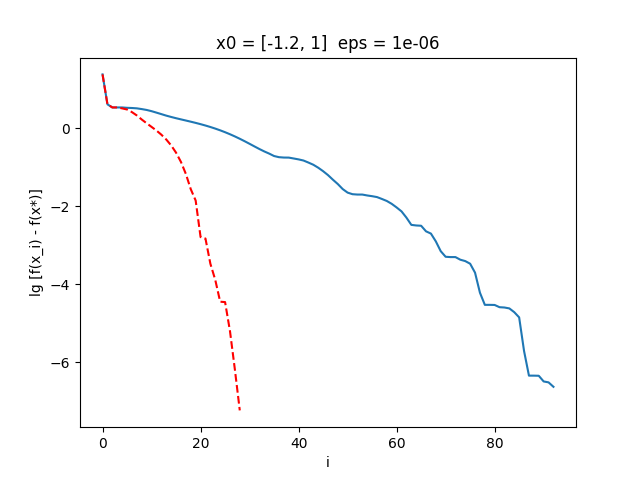
\includegraphics[width=0.9\linewidth]{Figure_1} \\
	\end{minipage}
	\hfill
	\begin{minipage}[h]{0.47\linewidth}
		\center{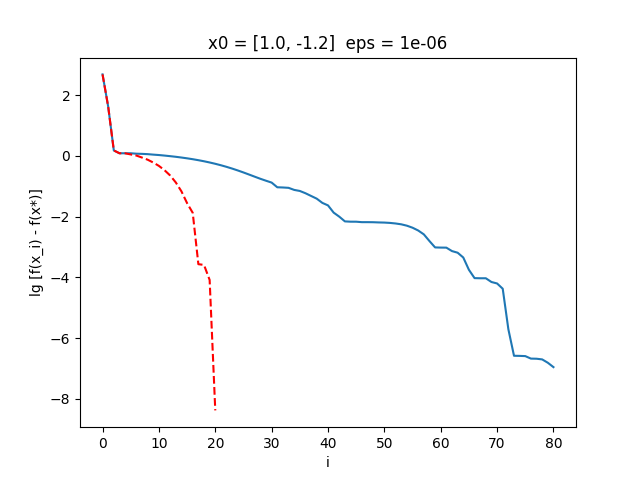
\includegraphics[width=0.9\linewidth]{Figure_1_1}} \\
	\end{minipage}
	\vfill
	\begin{minipage}[h]{0.47\linewidth}
		\center{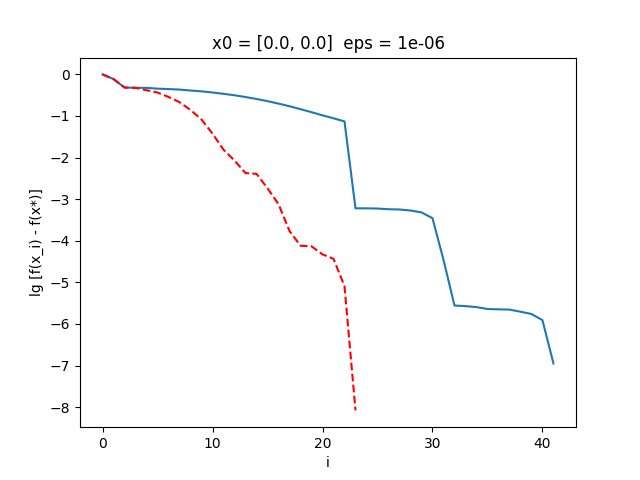
\includegraphics[width=0.9\linewidth]{Figure_1_2}}  \\
	\end{minipage}
	\hfill
	\begin{minipage}[h]{0.47\linewidth}
		\center{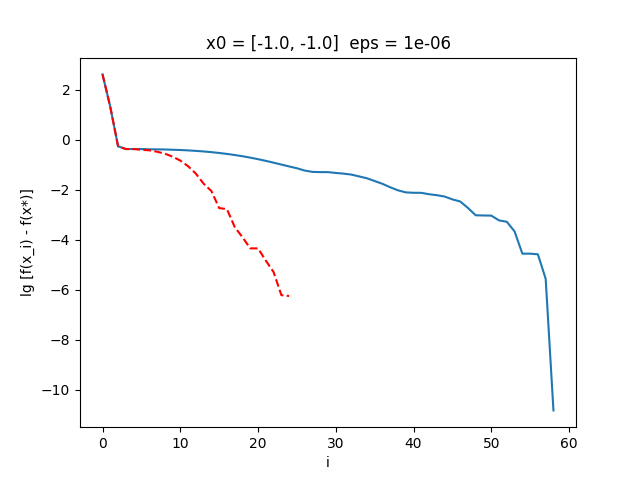
\includegraphics[width=0.9\linewidth]{Figure_1_3}}  \\
	\end{minipage}
\end{sidewaysfigure}


\rotatebox{90}{
	\begin{minipage}{1.5\linewidth}
		\begin{table}[H]
		\caption{}
			\begin{center}
				\begin{tabular}{|c|c|c|c|c|c|c|}
					\hline
					$\varepsilon$ & $x_0$ & $f(x_0)$ & Метод мінімізації & $x^* \text{ - отриманий розв'язок} $  & $f(x^*)$ & Кількість ітерацій \\
					\hline
					\multirow{8}{*}{$10^{-8}$}	& \multirow{2}{*}{[-1.2, 1]} & \multirow{2}{*}{24.2} & 4 кроковий & [ 0.99999  0.99999] & 0.0 & 98 \\
					\hhline{~~~----} & & & 3 кроковий & [ 0.99997  0.99994] & 0.0 & 35 \\
					\hhline{~------}
					& \multirow{2}{*}{[1.0, -1.2]} & \multirow{2}{*}{484.0} & 4 кроковий & [ 1.       0.99999] & 0.0 & 32 \\
					\hhline{~~~----} & & & 3 кроковий & [ 1.  1.] & 0.0 & 25 \\
					\hhline{~------}
					& \multirow{2}{*}{[0.0, 0.0]} & \multirow{2}{*}{1.0} & 4 кроковий & [ 0.99993  0.99985] & 0.0 & 24 \\
					\hhline{~~~----} & & & 3 кроковий & [ 1.  1.] & 0.0 & 19 \\
					\hhline{~------}
					& \multirow{2}{*}{[-1.0, -1.0]} & \multirow{2}{*}{404.0} & 4 кроковий & [ 0.99998  0.99996] & 0.0 & 20 \\
					\hhline{~~~----} & & & 3 кроковий & [ 1.  1.] & 0.0 & 16 \\
					\hline	
				\end{tabular}
			\end{center}
		\end{table}
\end{minipage}} 

\begin{sidewaysfigure}
\centering
\caption{}
	\begin{minipage}[h]{0.47\linewidth}
		\center{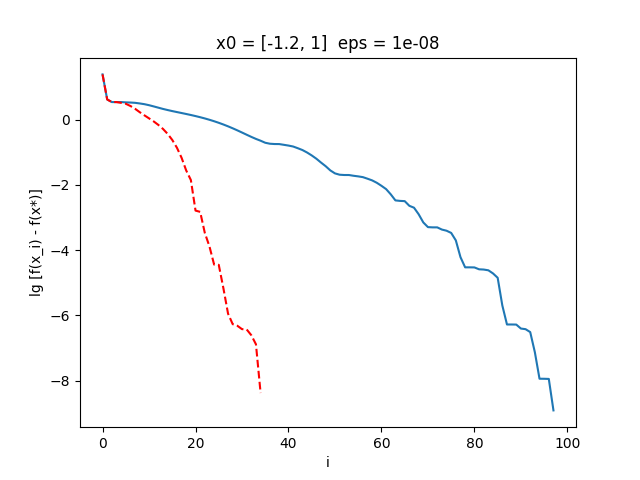
\includegraphics[width=0.9\linewidth]{Figure_1_1_1} \\
	\end{minipage}
	\hfill
	\begin{minipage}[h]{0.47\linewidth}
		\center{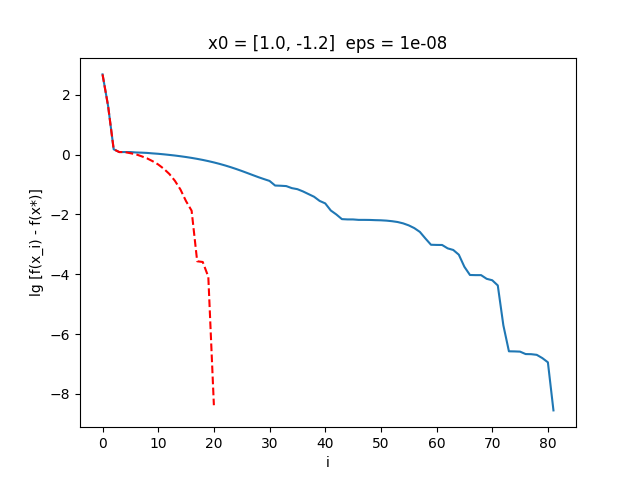
\includegraphics[width=0.9\linewidth]{Figure_1_1_2}} \\
	\end{minipage}
	\vfill
	\begin{minipage}[h]{0.47\linewidth}
		\center{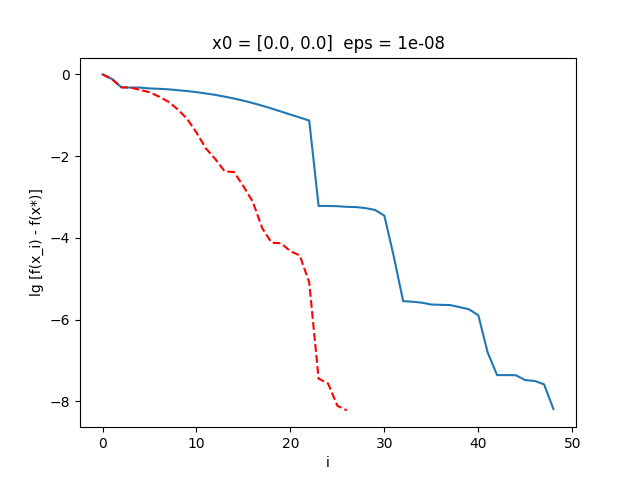
\includegraphics[width=0.9\linewidth]{Figure_1_1_3}}  \\
	\end{minipage}
	\hfill
	\begin{minipage}[h]{0.47\linewidth}
		\center{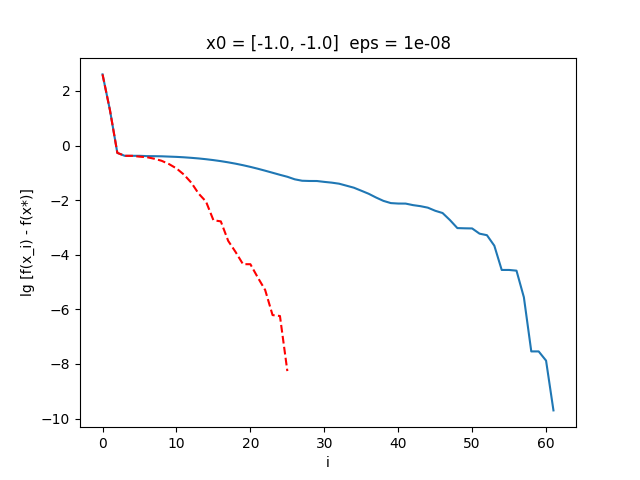
\includegraphics[width=0.9\linewidth]{Figure_1_1_4}}  \\
	\end{minipage}
\end{sidewaysfigure}

\rotatebox{90}{
	\begin{minipage}{1.55\linewidth}
	    \begin{example}
        	$$\phi(x) = \left(x_{1} + 10 x_{2}\right)^{2} + 10 \left(x_{1} - x_{4}\right)^{4} + \left(x_{2} - 2 x_{3}\right)^{4} + 5 \left(x_{3} - x_{4}\right)^{2}$$
        	Точний розв'язок задачі: x* = [0, 0, 0, 0] f* = 0
        \end{example}
		\begin{table}[H]
		\caption{}
			\begin{center}
				\begin{tabular}{|c|c|c|c|c|c|c|}
					\hline
					$\varepsilon$ & $x_0$ & $f(x_0)$ & Метод мінімізації & $x^* \text{ - отриманий розв'язок} $  & $f(x^*)$ & Кількість ітерацій \\
					\hline
				    \multirow{8}{*}{$10^{-6}$} & \multirow{2}{*}{[3, -1, 0, 1]} & \multirow{2}{*}{215} & 4 кроковий & [ 0.04999 -0.00496  0.03379  0.03432] & 3e-05 & 36 \\
				    \hhline{~~~----} & & & 3 кроковий & [ 0.0008  -0.00008 -0.00348 -0.00348] & 0.0 & 36 \\
				    \hhline{~------}
				    & \multirow{2}{*}{[1, 1, 1, 1]} & \multirow{2}{*}{122} & 4 кроковий & [-0.06942  0.00694 -0.04062 -0.04114] & 7e-05 & 43 \\
				    \hhline{~~~----} & & & 3 кроковий & [-0.04808  0.00482 -0.02532 -0.02525] & 1e-05 & 21 \\
				    \hhline{~------}
				    & \multirow{2}{*}{[-1.0, 1.0, -1.0, 1.0]} & \multirow{2}{*}{342.0} & 4 кроковий & [-0.08631  0.00862 -0.04842 -0.04857] & 0.00014 & 38 \\
				    \hhline{~~~----} & & & 3 кроковий & [ 0.00402 -0.00041 -0.01603 -0.01611] & 0.0 & 29 \\
				    \hhline{~------}
				    & \multirow{2}{*}{[0.0, 2.0, -1.0, 1.0]} & \multirow{2}{*}{686.0} & 4 кроковий & [ 0.00241 -0.00024  0.00156  0.00154] & 0.0 & 44 \\
				    \hhline{~~~----} & & & 3 кроковий & [-0.03611  0.00363 -0.00961 -0.00963] & 1e-05 & 27 \\
					\hline	
				\end{tabular}
			\end{center}
		\end{table}
\end{minipage}} 

\begin{sidewaysfigure}
\centering
\caption{}
	\begin{minipage}[h]{0.47\linewidth}
		\center{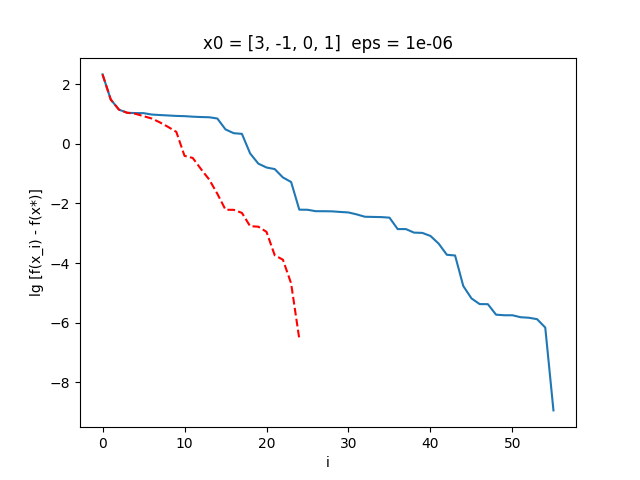
\includegraphics[width=0.9\linewidth]{Figure_2_1} \\
	\end{minipage}
	\hfill
	\begin{minipage}[h]{0.47\linewidth}
		\center{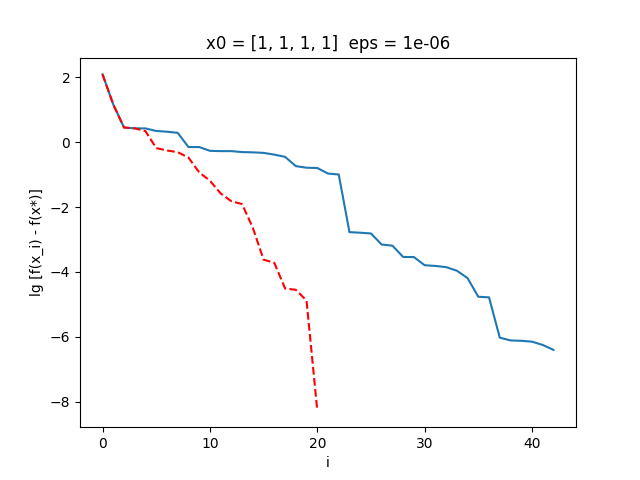
\includegraphics[width=0.9\linewidth]{Figure_2_2}} \\
	\end{minipage}
	\vfill
	\begin{minipage}[h]{0.47\linewidth}
		\center{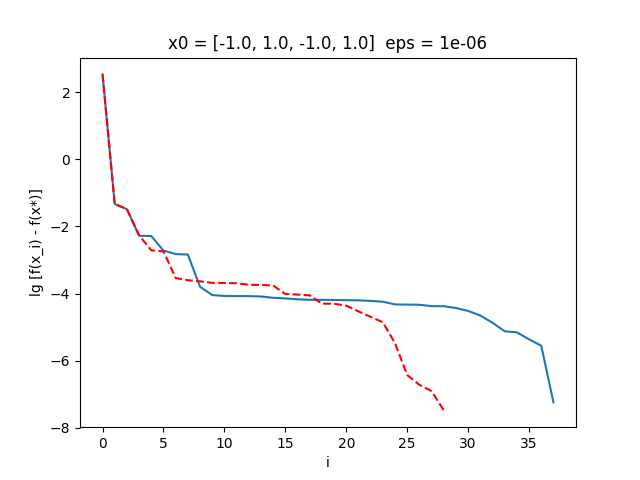
\includegraphics[width=0.9\linewidth]{Figure_2_3}}  \\
	\end{minipage}
	\hfill
	\begin{minipage}[h]{0.47\linewidth}
		\center{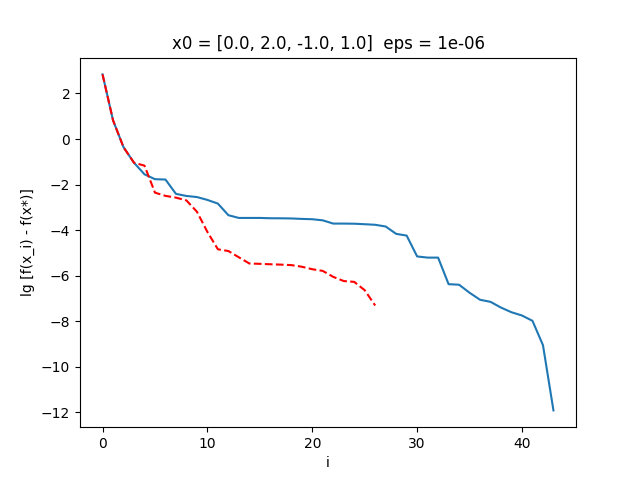
\includegraphics[width=0.9\linewidth]{Figure_2_4}}  \\
	\end{minipage}
\end{sidewaysfigure}

\rotatebox{90}{
	\begin{minipage}{1.55\linewidth}
		\begin{table}[H]
		\caption{}
			\begin{center}
				\begin{tabular}{|c|c|c|c|c|c|c|}
					\hline
					$\varepsilon$ & $x_0$ & $f(x_0)$ & Метод мінімізації & $x^* \text{ - отриманий розв'язок} $  & $f(x^*)$ & Кількість ітерацій \\
					\hline
					\multirow{8}{*}{$10^{-8}$} & \multirow{2}{*}{[3, -1, 0, 1]} & \multirow{2}{*}{215} & 4 кроковий & [-0.02558  0.00256 -0.01165 -0.01175] & 0.0 & 56 \\
					\hhline{~~~----} & & & 3 кроковий & [ 0.00019 -0.00002 -0.00241 -0.00241] & 0.0 & 34 \\
					\hhline{~------}
					& \multirow{2}{*}{[1, 1, 1, 1]} & \multirow{2}{*}{122} & 4 кроковий & [ 0.00081 -0.00008 -0.00795 -0.00794] & 0.0 & 106 \\
					\hhline{~~~----} & & & 3 кроковий & [-0.02441  0.00244 -0.01503 -0.01505] & 0.0 & 37 \\
					\hhline{~------}
					& \multirow{2}{*}{[-1.0, 1.0, -1.0, 1.0]} & \multirow{2}{*}{342.0} & 4 кроковий & [ 0.00905 -0.0009  -0.00682 -0.00667] & 0.0 & 83 \\
					\hhline{~~~----} & & & 3 кроковий & [-0.00833  0.00083 -0.00384 -0.00385] & 0.0 & 44 \\
					\hhline{~------}
					& \multirow{2}{*}{[0.0, 2.0, -1.0, 1.0]} & \multirow{2}{*}{686.0} & 4 кроковий & [ 0.00071 -0.00007  0.00963  0.00962] & 0.0 & 40 \\
					\hhline{~~~----} & & & 3 кроковий & [ 0.00041 -0.00004 -0.00281 -0.00281] & 0.0 & 62 \\
					\hline	
				\end{tabular}
			\end{center}
		\end{table}
\end{minipage}} 

\begin{sidewaysfigure}
\centering
\caption{}
	\begin{minipage}[h]{0.47\linewidth}
		\center{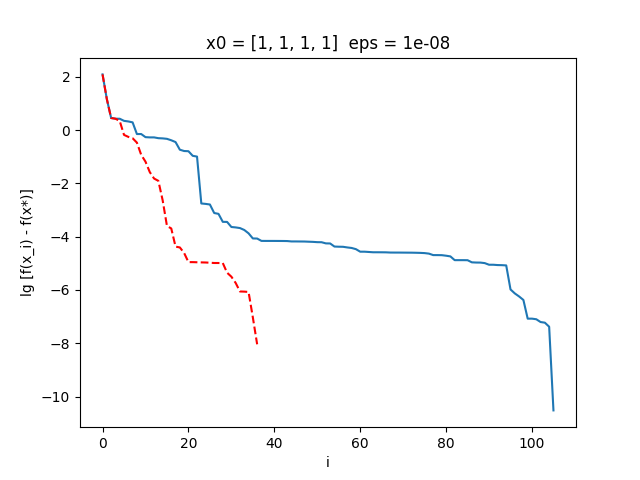
\includegraphics[width=0.9\linewidth]{Figure_2_1_4} \\
	\end{minipage}
	\hfill
	\begin{minipage}[h]{0.47\linewidth}
		\center{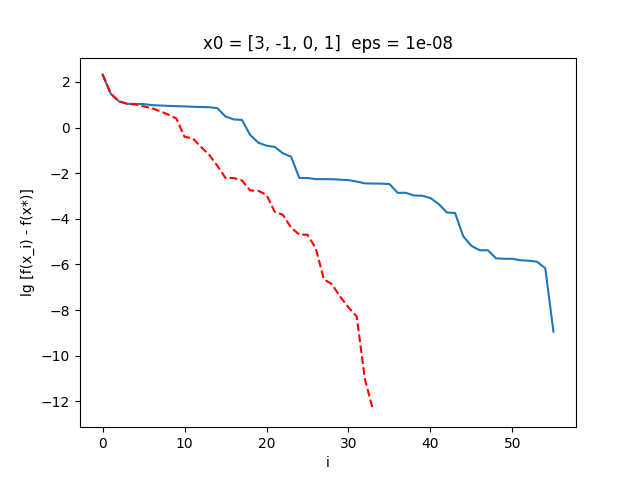
\includegraphics[width=0.9\linewidth]{Figure_2_1_3}} \\
	\end{minipage}
	\vfill
	\begin{minipage}[h]{0.47\linewidth}
		\center{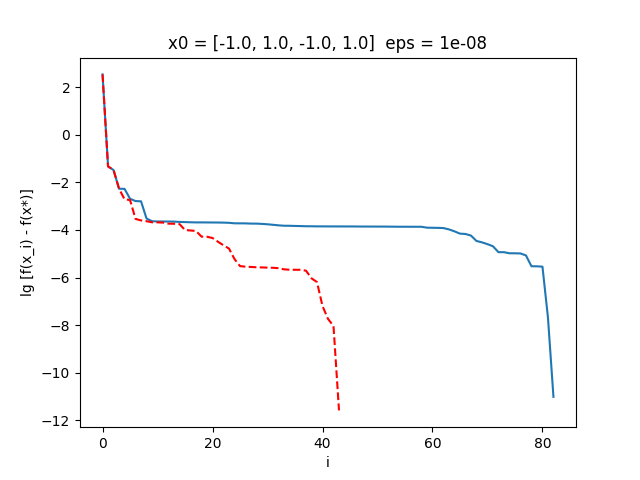
\includegraphics[width=0.9\linewidth]{Figure_2_1_2}}  \\
	\end{minipage}
	\hfill
	\begin{minipage}[h]{0.47\linewidth}
		\center{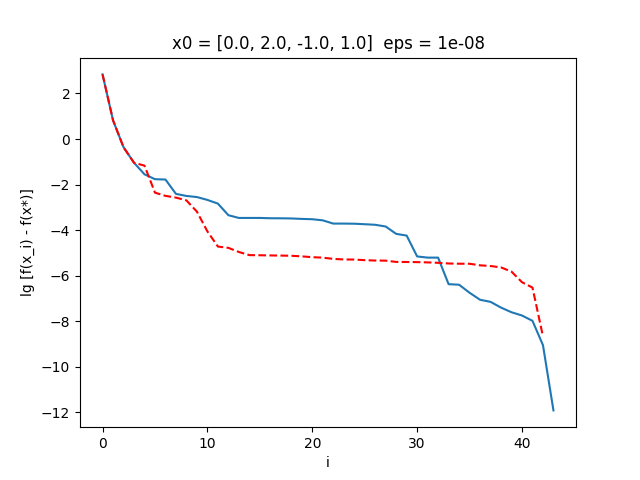
\includegraphics[width=0.9\linewidth]{Figure_2_1_1}}  \\
	\end{minipage}
\end{sidewaysfigure}



\rotatebox{90}{
	\begin{minipage}{1.5\linewidth}
	    \begin{example}
        	$$\phi(x) = \left(x_{1} + x_{2}^{2} - 7\right)^{2} + \left(x_{1}^{2} + x_{2} - 11\right)^{2}$$
        	Точний розв'язок задачі:  x* = [3, 2] f* = 0
        \end{example}
		\begin{table}[H]
		\caption{}
			\begin{center}
				\begin{tabular}{|c|c|c|c|c|c|c|}
					\hline
					$\varepsilon$ & $x_0$ & $f(x_0)$ & Метод мінімізації & $x^* \text{ - отриманий розв'язок} $  & $f(x^*)$ & Кількість ітерацій \\
					\hline
					\multirow{8}{*}{$10^{-6}$} & \multirow{2}{*}{[1, 1]} & \multirow{2}{*}{106} & 4 кроковий & [ 3.  2.] & 0.0 & 11 \\
					\hhline{~~~----} & & & 3 кроковий & [ 3.  2.] & 0.0 & 9 \\
					\hhline{~------}
					& \multirow{2}{*}{[1.0, 4.0]} & \multirow{2}{*}{136.0} & 4 кроковий & [ 3.  2.] & 0.0 & 17 \\
					\hhline{~~~----} & & & 3 кроковий & [ 3.00011  2.00001] & 0.0 & 9 \\
					\hhline{~------}
					& \multirow{2}{*}{[0.0, 0.0]} & \multirow{2}{*}{170.0} & 4 кроковий & [ 2.99991  1.99991] & 0.0 & 30 \\
					\hhline{~~~----} & & & 3 кроковий & [ 2.99999  2.00016] & 0.0 & 19 \\
					\hhline{~------}
					& \multirow{2}{*}{[2.5, 2.5]} & \multirow{2}{*}{8.125} & 4 кроковий & [ 3.  2.] & 0.0 & 13 \\
					\hhline{~~~----} & & & 3 кроковий & [ 2.99998  2.00004] & 0.0 & 7 \\
					\hline	
				\end{tabular}
			\end{center}
		\end{table}
\end{minipage}} 

\begin{sidewaysfigure}
\centering
\caption{}
	\begin{minipage}[h]{0.47\linewidth}
		\center{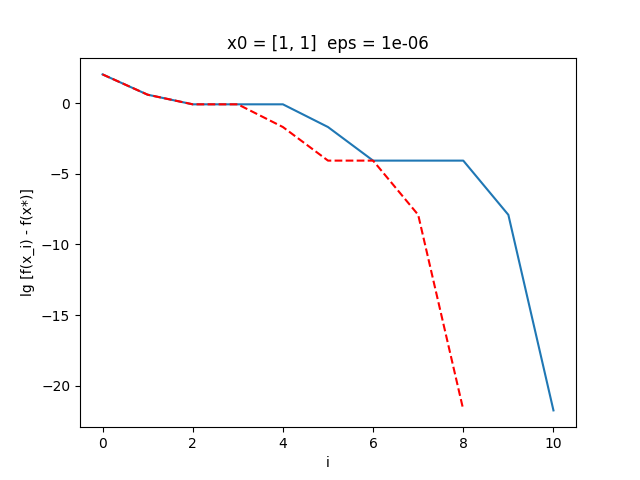
\includegraphics[width=0.9\linewidth]{Figure_3_1} \\
	\end{minipage}
	\hfill
	\begin{minipage}[h]{0.47\linewidth}
		\center{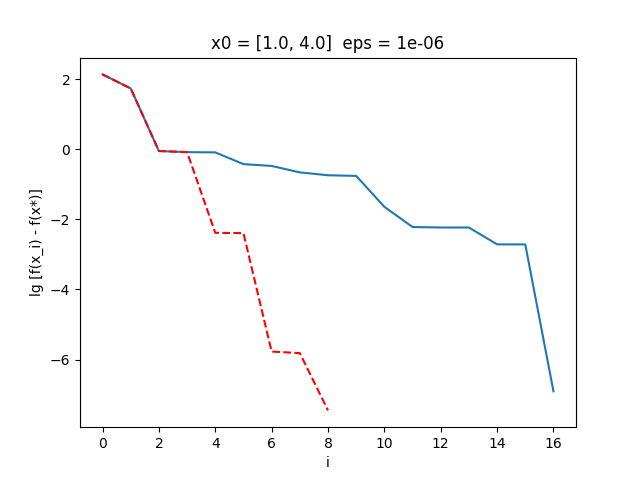
\includegraphics[width=0.9\linewidth]{Figure_3_2}} \\
	\end{minipage}
	\vfill
	\begin{minipage}[h]{0.47\linewidth}
		\center{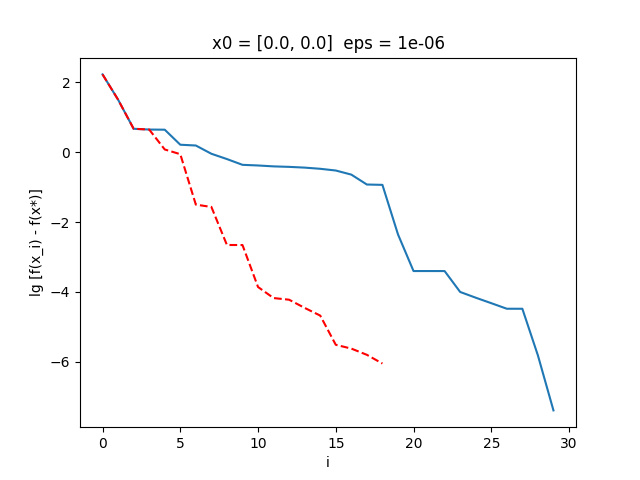
\includegraphics[width=0.9\linewidth]{Figure_3_3}}  \\
	\end{minipage}
	\hfill
	\begin{minipage}[h]{0.47\linewidth}
		\center{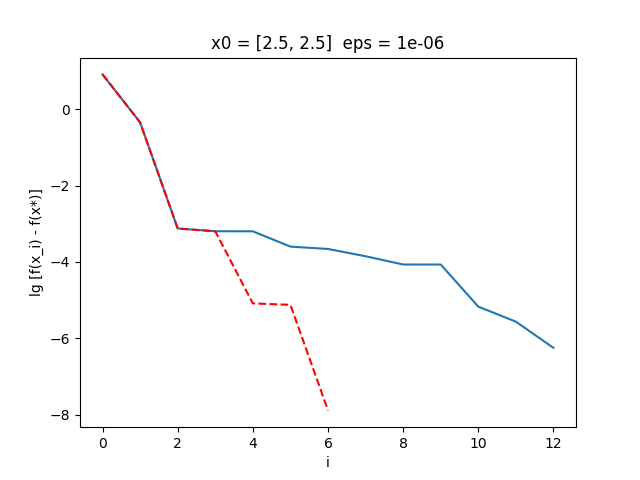
\includegraphics[width=0.9\linewidth]{Figure_3_40}}  \\
	\end{minipage}
\end{sidewaysfigure}

\rotatebox{90}{
	\begin{minipage}{1.5\linewidth}
		\begin{table}[H]
		\caption{}
			\begin{center}
				\begin{tabular}{|c|c|c|c|c|c|c|}
					\hline
					$\varepsilon$ & $x_0$ & $f(x_0)$ & Метод мінімізації & $x^* \text{ - отриманий розв'язок} $  & $f(x^*)$ & Кількість ітерацій \\
					\hline
					\multirow{8}{*}{$10^{-8}$} & \multirow{2}{*}{[1, 1]} & \multirow{2}{*}{106} & 4 кроковий & [ 3.  2.] & 0.0 & 12 \\
					\hhline{~~~----} & & & 3 кроковий & [ 3.  2.] & 0.0 & 10 \\
					\hhline{~------}
					& \multirow{2}{*}{[1.0, 4.0]} & \multirow{2}{*}{136.0} & 4 кроковий & [ 3.  2.] & 0.0 & 18 \\
					\hhline{~~~----} & & & 3 кроковий & [ 2.99998  2.00003] & 0.0 & 12 \\
					\hhline{~------}
					& \multirow{2}{*}{[0.0, 0.0]} & \multirow{2}{*}{170.0} & 4 кроковий & [ 2.99998  2.     ] & 0.0 & 35 \\
					\hhline{~~~----} & & & 3 кроковий & [ 2.99999  1.99998] & 0.0 & 23 \\
					\hhline{~------}
					& \multirow{2}{*}{[2.5, 2.5]} & \multirow{2}{*}{8.125} & 4 кроковий & [ 3.  2.] & 0.0 & 14 \\
					\hhline{~~~----} & & & 3 кроковий & [ 3.00001  2.00001] & 0.0 & 9 \\
					\hline	
				\end{tabular}
			\end{center}
		\end{table}
\end{minipage}} 

\begin{sidewaysfigure}
\centering
\caption{}
	\begin{minipage}[h]{0.47\linewidth}
		\center{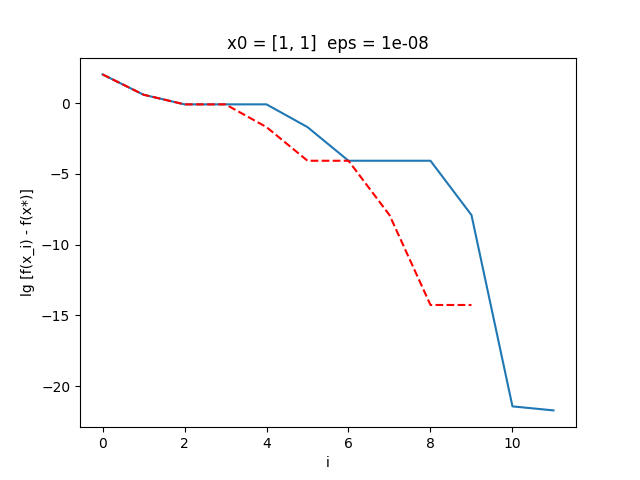
\includegraphics[width=0.9\linewidth]{Figure_3_1_1} \\
	\end{minipage}
	\hfill
	\begin{minipage}[h]{0.47\linewidth}
		\center{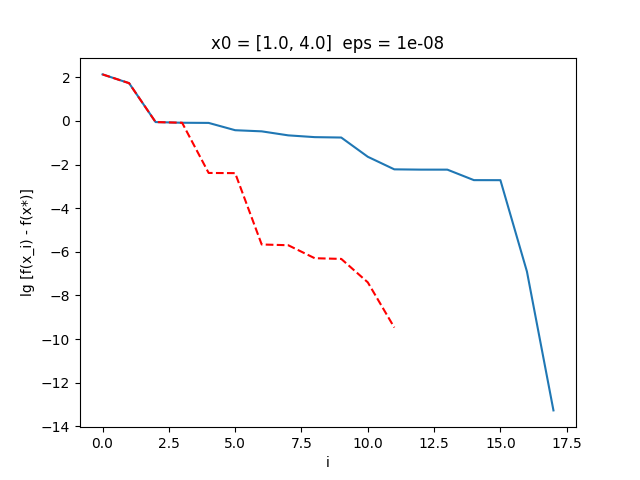
\includegraphics[width=0.9\linewidth]{Figure_3_1_2}} \\
	\end{minipage}
	\vfill
	\begin{minipage}[h]{0.47\linewidth}
		\center{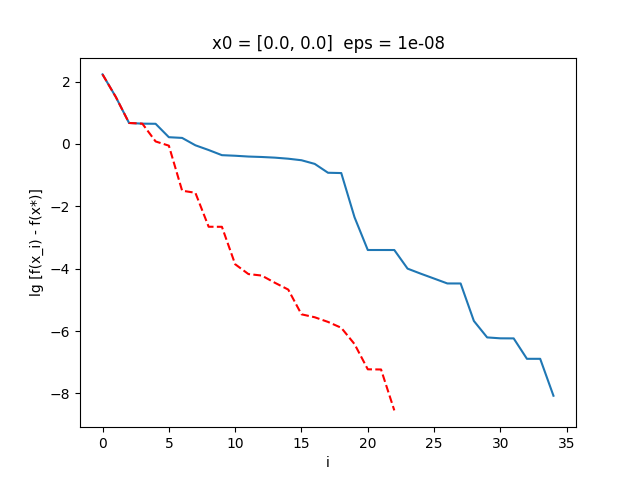
\includegraphics[width=0.9\linewidth]{Figure_3_4}}  \\
	\end{minipage}
	\hfill
	\begin{minipage}[h]{0.47\linewidth}
		\center{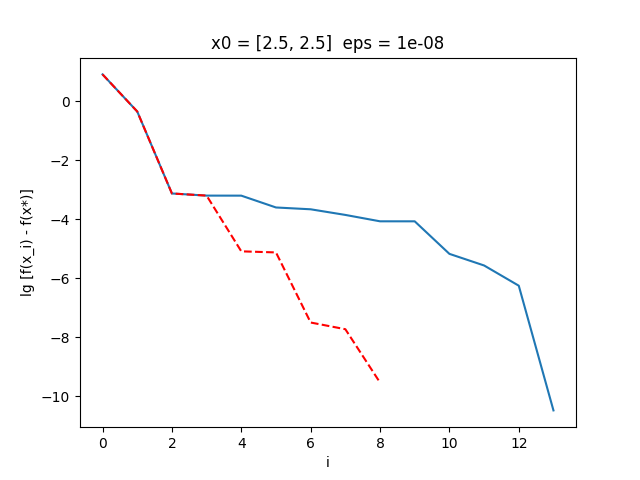
\includegraphics[width=0.9\linewidth]{Figure_3_1_4}}  \\
	\end{minipage}
\end{sidewaysfigure}


\rotatebox{90}{
	\begin{minipage}{1.5\linewidth}
    	\begin{example}
        	$$\phi(x) = \left(x_{1}^{2} + 12 x_{2} - 1\right)^{2} + \left(49 x_{1}^{2} + 84 x_{1} + 49 x_{2}^{2} + 2324 x_{2} - 681\right)^{2} $$
        	Точний розв'язок задачі: x* = [0.28581, 0.27936] f* = 5.9225
        \end{example}
		\begin{table}[H]
		\caption{}
			\begin{center}
				\begin{tabular}{|c|c|c|c|c|c|c|}
					\hline
					$\varepsilon$ & $x_0$ & $f(x_0)$ & Метод мінімізації & $x^* \text{ - отриманий розв'язок} $  & $f(x^*)$ & Кількість ітерацій \\
					\hline
					\multirow{8}{*}{$10^{-6}$} & \multirow{2}{*}{[1, 1]} & \multirow{2}{*}{3330769} & 4 кроковий & [ 0.28582  0.27933] & 5.92256 & 88 \\
					\hhline{~~~----} & & & 3 кроковий & [ 0.28582  0.27933] & 5.92256 & 26 \\
					\hhline{~------}
					& \multirow{2}{*}{[0.0, 0.0]} & \multirow{2}{*}{463762.0} & 4 кроковий & [ 0.28583  0.27933] & 5.92256 & 70 \\
					\hhline{~~~----} & & & 3 кроковий & [ 0.2858   0.27933] & 5.92256 & 22 \\
					\hhline{~------}
					& \multirow{2}{*}{[-5.0, -7.0]} & \multirow{2}{*}{188873649.0} & 4 кроковий & [ 0.28581  0.27933] & 5.92256 & 91 \\
					\hhline{~~~----} & & & 3 кроковий & [ 0.28581  0.27933] & 5.92256 & 69 \\
					\hhline{~------}
					& \multirow{2}{*}{[0.2, 0.3]} & \multirow{2}{*}{1556.9665} & 4 кроковий & [ 0.28583  0.27933] & 5.92256 & 41 \\
					\hhline{~~~----} & & & 3 кроковий & [ 0.28587  0.27932] & 5.92256 & 21 \\
					\hline	
				\end{tabular}
			\end{center}
		\end{table}
\end{minipage}} 

\begin{sidewaysfigure}
\centering
\caption{}
	\begin{minipage}[h]{0.47\linewidth}
		\center{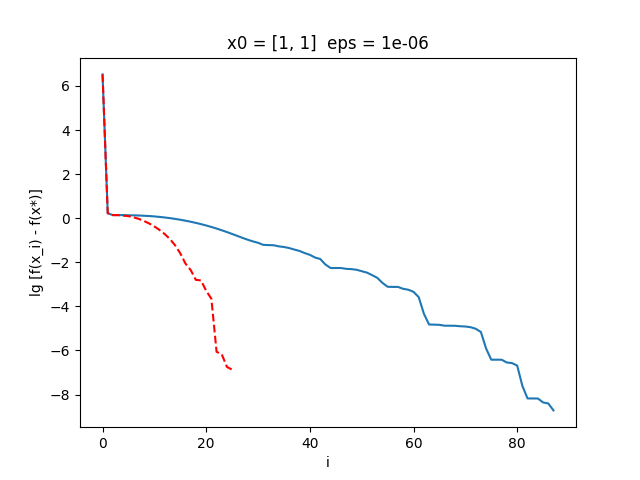
\includegraphics[width=0.9\linewidth]{Figure_4_1} \\
	\end{minipage}
	\hfill
	\begin{minipage}[h]{0.47\linewidth}
		\center{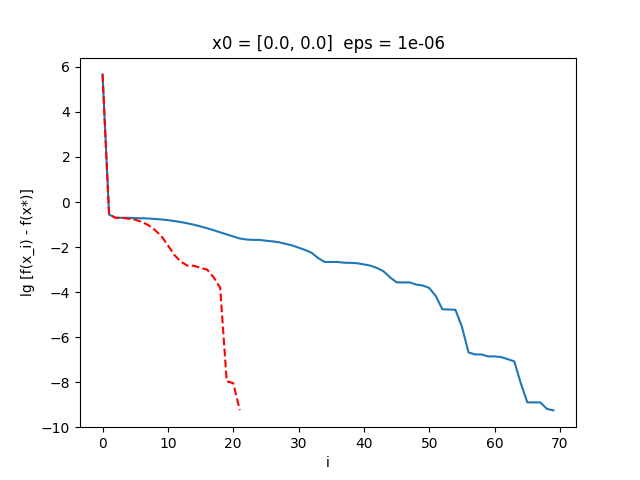
\includegraphics[width=0.9\linewidth]{Figure_4_2}} \\
	\end{minipage}
	\vfill
	\begin{minipage}[h]{0.47\linewidth}
		\center{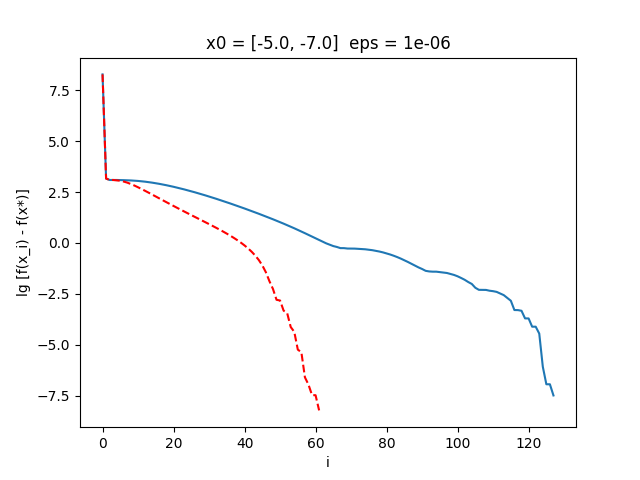
\includegraphics[width=0.9\linewidth]{Figure_4_3}}  \\
	\end{minipage}
	\hfill
	\begin{minipage}[h]{0.47\linewidth}
		\center{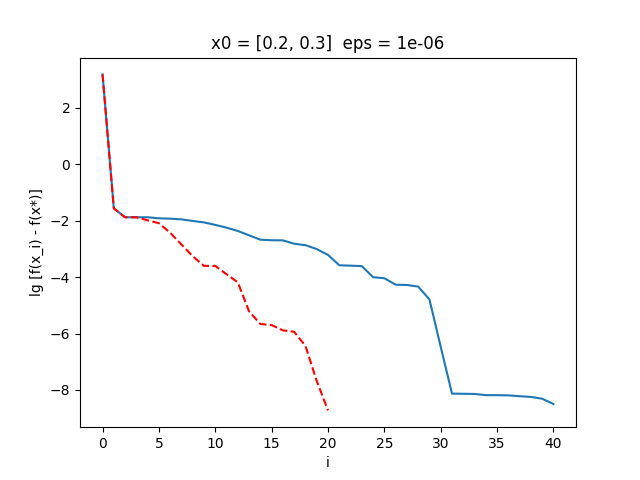
\includegraphics[width=0.9\linewidth]{Figure_4_4}}  \\
	\end{minipage}
\end{sidewaysfigure}

\rotatebox{90}{
	\begin{minipage}{1.5\linewidth}
		\begin{table}[H]
		\caption{}
			\begin{center}
				\begin{tabular}{|c|c|c|c|c|c|c|}
					\hline
					$\varepsilon$ & $x_0$ & $f(x_0)$ & Метод мінімізації & $x^* \text{ - отриманий розв'язок} $  & $f(x^*)$ & Кількість ітерацій \\
					\hline
					\multirow{8}{*}{$10^{-8}$} & \multirow{2}{*}{[1, 1]} & \multirow{2}{*}{3330769} & 4 кроковий & [ 0.28581  0.27933] & 5.92256 & 91 \\
					\hhline{~~~----} & & & 3 кроковий & [ 0.28582  0.27933] & 5.92256 & 27 \\
					\hhline{~------}
					& \multirow{2}{*}{[0.0, 0.0]} & \multirow{2}{*}{463762.0} & 4 кроковий & [ 0.28581  0.27933] & 5.92256 & 73 \\
					\hhline{~~~----} & & & 3 кроковий & [ 0.28582  0.27933] & 5.92256 & 25 \\
					\hhline{~------}
					& \multirow{2}{*}{[-5.0, -7.0]} & \multirow{2}{*}{188873649.0} & 4 кроковий & [ 0.28581  0.27933] & 5.92256 & 152 \\
					\hhline{~~~----} & & & 3 кроковий & [ 0.28581  0.27933] & 5.92256 & 64 \\
					\hhline{~------}
					& \multirow{2}{*}{[0.2, 0.3]} & \multirow{2}{*}{1556.9665} & 4 кроковий & [ 0.28581  0.27933] & 5.92256 & 15 \\
					\hhline{~~~----} & & & 3 кроковий & [ 0.28581  0.27933] & 5.92256 & 12 \\
					\hline	
				\end{tabular}
			\end{center}
		\end{table}
\end{minipage}} 

\begin{sidewaysfigure}
\centering
\caption{}
	\begin{minipage}[h]{0.47\linewidth}
		\center{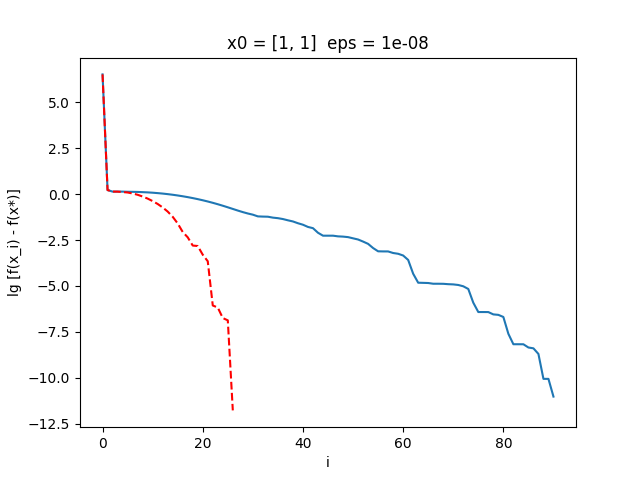
\includegraphics[width=0.9\linewidth]{Figure_4_1_1} \\
	\end{minipage}
	\hfill
	\begin{minipage}[h]{0.47\linewidth}
		\center{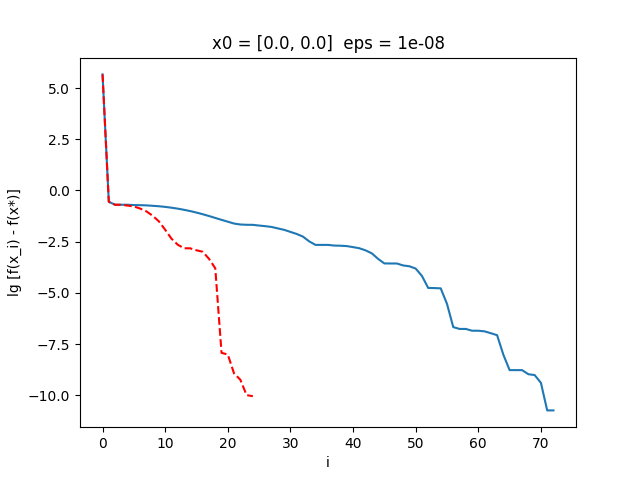
\includegraphics[width=0.9\linewidth]{Figure_4_1_2}} \\
	\end{minipage}
	\vfill
	\begin{minipage}[h]{0.47\linewidth}
		\center{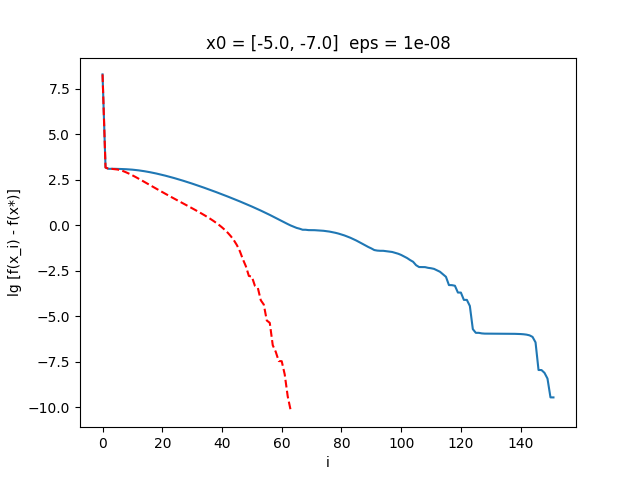
\includegraphics[width=0.9\linewidth]{Figure_4_1_3}}  \\
	\end{minipage}
	\hfill
	\begin{minipage}[h]{0.47\linewidth}
		\center{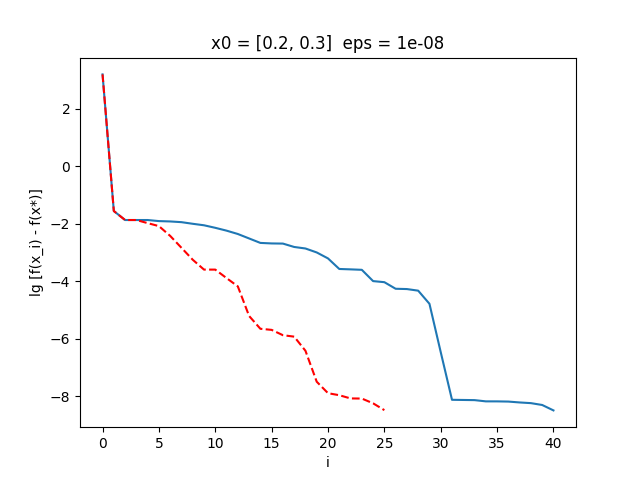
\includegraphics[width=0.9\linewidth]{Figure_4_1_4}}  \\
	\end{minipage}
\end{sidewaysfigure}

\rotatebox{90}{
	\begin{minipage}{1.5\linewidth}
    	\begin{example}
        	$$\phi(x) = \left(- x_{1} + 1\right)^{2} + \left(- x_{2} + 1\right)^{2} + 100 \left(x_{3} - \left(\frac{x_{1}}{2} + \frac{x_{2}}{2}\right)^{2}\right)^{2}$$
        	Точний розв'язок задачі: x* = [1, 1, 1] f* = 0
        \end{example}
		\begin{table}[H]
		\caption{}
			\begin{center}
				\begin{tabular}{|c|c|c|c|c|c|c|}
					\hline
					$\varepsilon$ & $x_0$ & $f(x_0)$ & Метод мінімізації & $x^* \text{ - отриманий розв'язок} $  & $f(x^*)$ & Кількість ітерацій \\
					\hline
					\multirow{8}{*}{$10^{-6}$} & \multirow{2}{*}{[-1.2, 2, 0]} & \multirow{2}{*}{8.4} & 4 кроковий & [ 0.99756  0.99819  0.99575] & 1e-05 & 67 \\
					\hhline{~~~----} & & & 3 кроковий & [ 1.00002  0.99978  0.99979] & 0.0 & 31 \\
					\hhline{~------}
					& \multirow{2}{*}{[0.0, 0.0, 0.0]} & \multirow{2}{*}{2.0} & 4 кроковий & [ 1.00009  1.00009  1.00018] & 0.0 & 51 \\
					\hhline{~~~----} & & & 3 кроковий & [ 1.00047  1.00047  1.00091] & 0.0 & 23 \\
					\hhline{~------}
					& \multirow{2}{*}{[0.0, 1.0, -1.2]} & \multirow{2}{*}{211.25} & 4 кроковий & [ 0.99745  1.00094  0.99839] & 1e-05 & 66 \\
					\hhline{~~~----} & & & 3 кроковий & [ 1.00443  0.99998  1.00444] & 2e-05 & 53 \\
					\hhline{~------}
					& \multirow{2}{*}{[2.3, 1.0, -0.3]} & \multirow{2}{*}{915.24062} & 4 кроковий & [ 1.0009   0.9995   1.00042] & 0.0 & 51 \\
					\hhline{~~~----} & & & 3 кроковий & [ 1.00005  0.99997  1.00002] & 0.0 & 24 \\
					\hline	
				\end{tabular}
			\end{center}
		\end{table}
\end{minipage}} 

\begin{sidewaysfigure}
\centering
\caption{}
	\begin{minipage}[h]{0.47\linewidth}
		\center{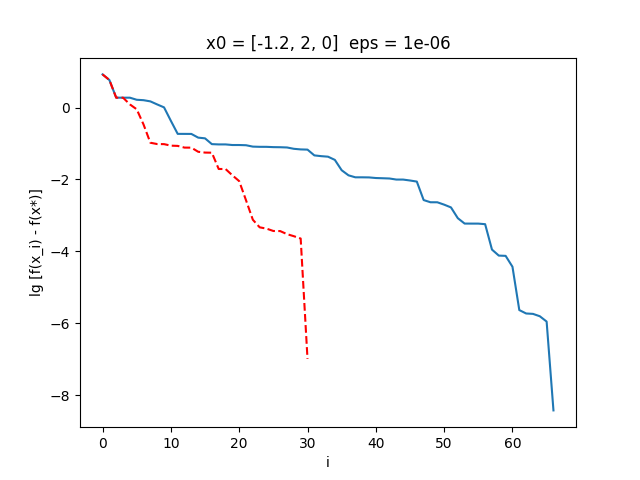
\includegraphics[width=0.9\linewidth]{Figure_5_1} \\
	\end{minipage}
	\hfill
	\begin{minipage}[h]{0.47\linewidth}
		\center{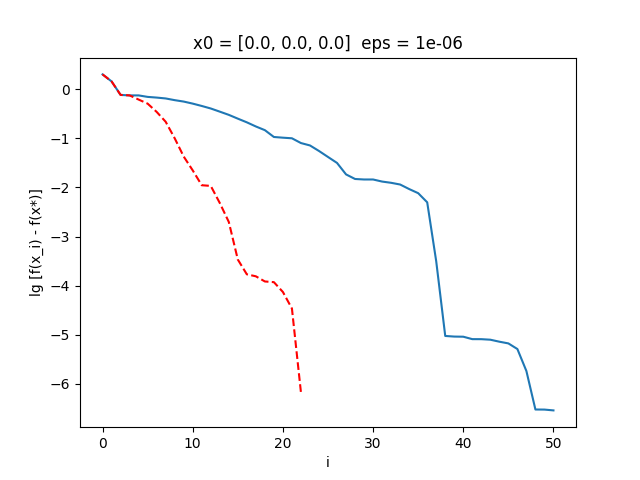
\includegraphics[width=0.9\linewidth]{Figure_5_2}} \\
	\end{minipage}
	\vfill
	\begin{minipage}[h]{0.47\linewidth}
		\center{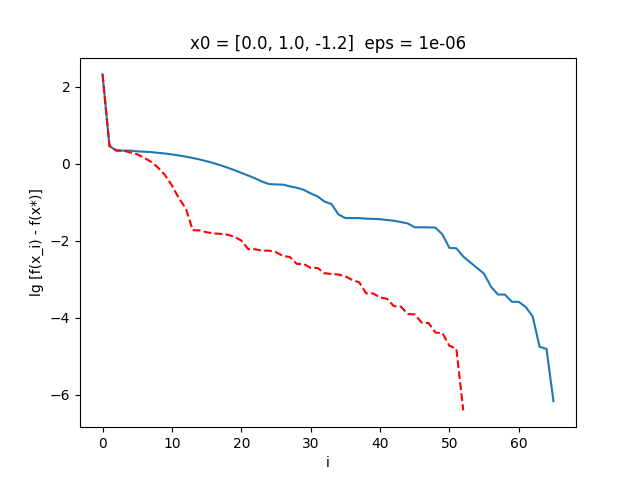
\includegraphics[width=0.9\linewidth]{Figure_5_3}}  \\
	\end{minipage}
	\hfill
	\begin{minipage}[h]{0.47\linewidth}
		\center{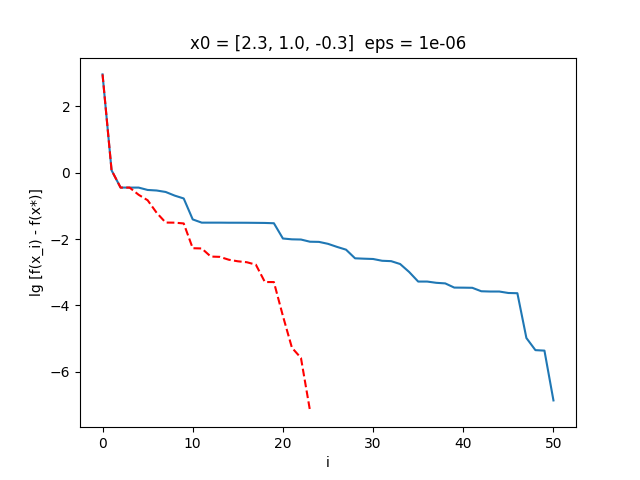
\includegraphics[width=0.9\linewidth]{Figure_5_4}}  \\
	\end{minipage}
\end{sidewaysfigure}

\rotatebox{90}{
	\begin{minipage}{1.5\linewidth}
		\begin{table}[H]
		\caption{}
			\begin{center}
				\begin{tabular}{|c|c|c|c|c|c|c|}
					\hline
					$\varepsilon$ & $x_0$ & $f(x_0)$ & Метод мінімізації & $x^* \text{ - отриманий розв'язок} $  & $f(x^*)$ & Кількість ітерацій \\
					\hline
					\multirow{8}{*}{$10^{-8}$} & \multirow{2}{*}{[-1.2, 2, 0]} & \multirow{2}{*}{8.4} & 4 кроковий & [ 1.00002  0.99975  0.99977] & 0.0 & 96 \\
					\hhline{~~~----} & & & 3 кроковий & [ 1.  1.  1.] & 0.0 & 33 \\
					\hhline{~------}
					& \multirow{2}{*}{[0.0, 0.0, 0.0]} & \multirow{2}{*}{2.0} & 4 кроковий & [ 1.  1.  1.] & 0.0 & 53 \\
					\hhline{~~~----} & & & 3 кроковий & [ 1.0004  1.0004  1.0008] & 0.0 & 26 \\
					\hhline{~------}
					& \multirow{2}{*}{[0.0, 1.0, -1.2]} & \multirow{2}{*}{211.25} & 4 кроковий & [ 1.00002  0.99996  0.99998] & 0.0 & 75 \\
					\hhline{~~~----} & & & 3 кроковий & [ 1.  1.  1.] & 0.0 & 57 \\
					\hhline{~------}
					& \multirow{2}{*}{[2.3, 1.0, -0.3]} & \multirow{2}{*}{915.24062} & 4 кроковий & [ 1.00093  1.00004  1.00097] & 0.0 & 63 \\
					\hhline{~~~----} & & & 3 кроковий & [ 1.00004  0.99996  1.     ] & 0.0 & 25 \\
					\hline	
				\end{tabular}
			\end{center}
		\end{table}
\end{minipage}} 

\begin{sidewaysfigure}
\centering
\caption{}
	\begin{minipage}[h]{0.47\linewidth}
		\center{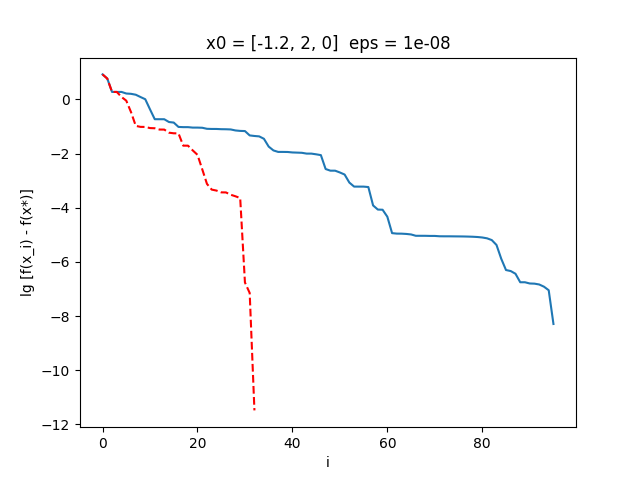
\includegraphics[width=0.9\linewidth]{Figure_5_1_1} \\
	\end{minipage}
	\hfill
	\begin{minipage}[h]{0.47\linewidth}
		\center{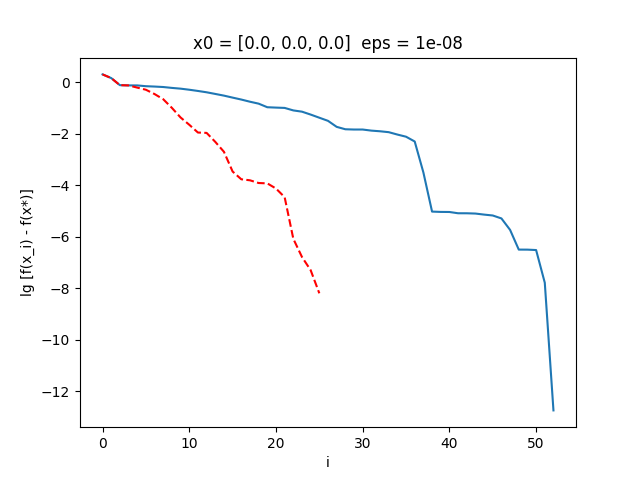
\includegraphics[width=0.9\linewidth]{Figure_5_1_2}} \\
	\end{minipage}
	\vfill
	\begin{minipage}[h]{0.47\linewidth}
		\center{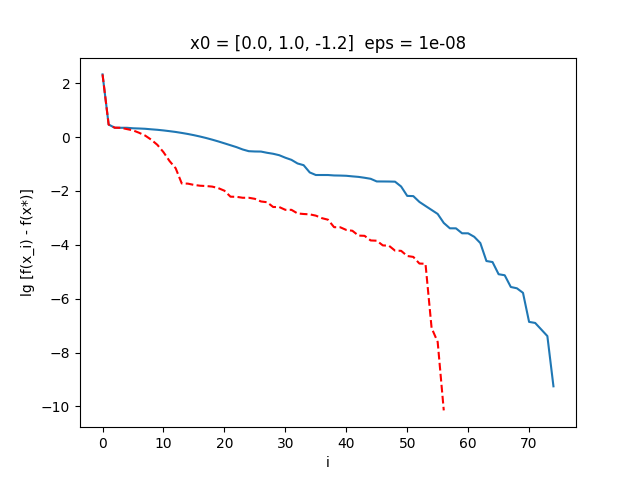
\includegraphics[width=0.9\linewidth]{Figure_5_1_3}}  \\
	\end{minipage}
	\hfill
	\begin{minipage}[h]{0.47\linewidth}
		\center{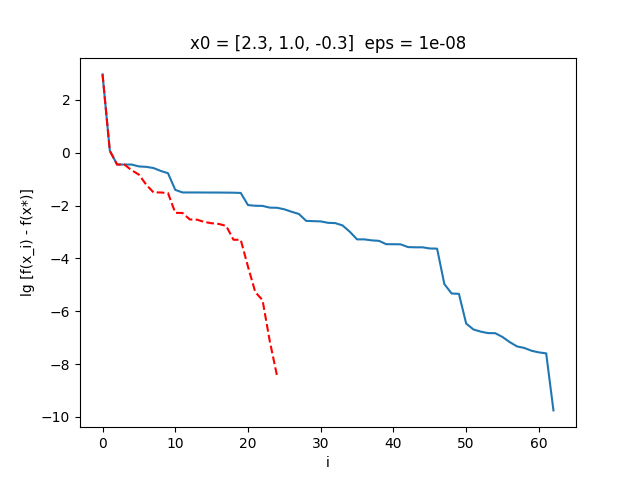
\includegraphics[width=0.9\linewidth]{Figure_5_1_4}}  \\
	\end{minipage}
\end{sidewaysfigure}

\rotatebox{90}{
	\begin{minipage}{1.5\linewidth}
    	\begin{example}
    	
    	
        	$\phi(x) = 1352.99 x_{1}^{2} - 70000.0 + \frac{319.28 x_{1}^{2} + 1.67 x_{2}^{2} + 0.008 x_{3}^{2}}{0.005 x_{4}^{2} + 1} +  \frac{416.31 x_{1}^{2} + 1.4 x_{2}^{2} + 0.005 x_{3}^{2}}{0.003 x_{4}^{2} + 1} + \frac{450.45 x_{1}^{2} + 0.94 x_{2}^{2} + 0.001 x_{3}^{2}}{0.002 x_{4}^{2} + 1} +$ \\
        	$ +  \frac{617.28 x_{1}^{2} + 0.99 x_{2}^{2} + 0.001 x_{3}^{2}}{0.001 x_{4}^{2} + 1} + \frac{608.27 x_{1}^{2} + 0.608272506082725 x_{2}^{2} + 0.0006 x_{3}^{2}}{0.001 x_{4}^{2} + 1} + \frac{894.46 x_{1}^{2} + 0.38 x_{2}^{2} + 0.00016 x_{3}^{2}}{0.0004 x_{4}^{2} + 1}$\\
        	Точний розв'язок задачі: x* = [0, 0, 0, 1] f* = -70000
        \end{example}
		\begin{table}[H]
		\caption{}
			\begin{center}
				\begin{tabular}{|c|c|c|c|c|c|c|}
					\hline
					$\varepsilon$ & $x_0$ & $f(x_0)$ & Метод мінімізації & $x^* \text{ - отриманий розв'язок} $  & $f(x^*)$ & Кількість ітерацій \\
					\hline
					\multirow{8}{*}{$10^{-6}$} & \multirow{2}{*}{[2.7, 90, 1500, 10]} & \multirow{2}{*}{28580.05} & 4 кроковий & [    0.13   -15.05  1495.2   331.4] & -69844 & 12 \\
					\hhline{~~~----} & & & 3 кроковий & [   -0.0008    25.86  1488.1   473.1] & -69930.4 & 26 \\
					\hhline{~------}
					& \multirow{2}{*}{[2, 140, 1707, 31]} & \multirow{2}{*}{-8899.54} & 4 кроковий & [    0.009   -28.76  1702.29   688.04] & -69957 & 24 \\
					\hhline{~~~----} & & & 3 кроковий & [    0.004   -35.7  1702.1   709.41] & -69956.5 & 15 \\
					\hhline{~------}
					& \multirow{2}{*}{[1, 1, 1, 1]} & \multirow{2}{*}{-65341} & 4 кроковий & [ 0.       0.00001  0.005 1.007] & -70000 & 8 \\
					\hhline{~~~----} & & & 3 кроковий & [-0.       0.00001  0.0015   1.006] & -70000 & 7 \\
					\hhline{~------}
					& \multirow{2}{*}{[-1, 0, 1, -1]} & \multirow{2}{*}{-65346.95} & 4 кроковий & [-0.00001  0.       0.00001 -1.00519] & -70000 & 4 \\
					\hhline{~~~----} & & & 3 кроковий & [ 0.       0.       0.      -1.0051] & -70000 & 4 \\
					\hline	
				\end{tabular}
			\end{center}
		\end{table}
\end{minipage}} 

\begin{sidewaysfigure}
\centering
\caption{}
	\begin{minipage}[h]{0.47\linewidth}
		\center{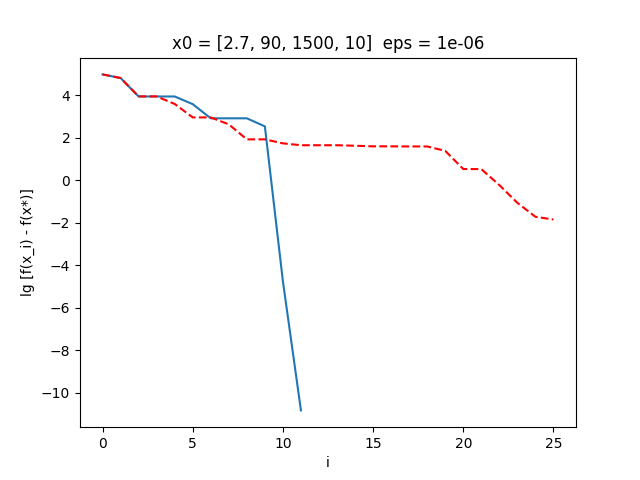
\includegraphics[width=0.9\linewidth]{Figure_6_1} \\
	\end{minipage}
	\hfill
	\begin{minipage}[h]{0.47\linewidth}
		\center{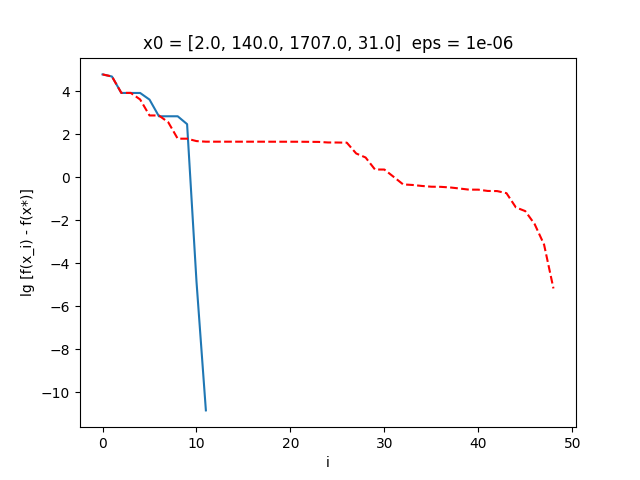
\includegraphics[width=0.9\linewidth]{Figure_6_2}} \\
	\end{minipage}
	\vfill
	\begin{minipage}[h]{0.47\linewidth}
		\center{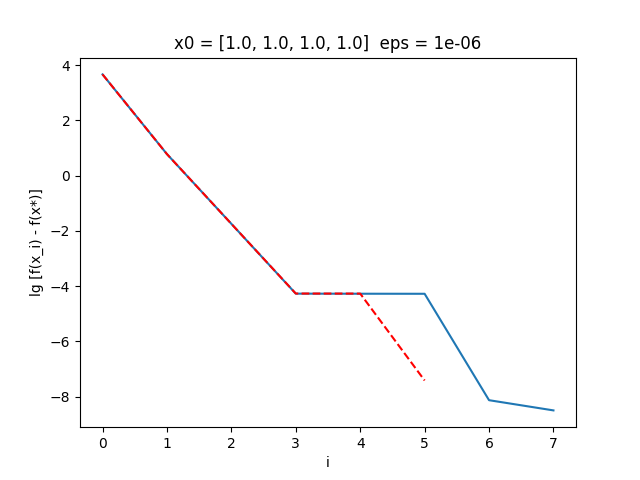
\includegraphics[width=0.9\linewidth]{Figure_6_3}}  \\
	\end{minipage}
	\hfill
	\begin{minipage}[h]{0.47\linewidth}
		\center{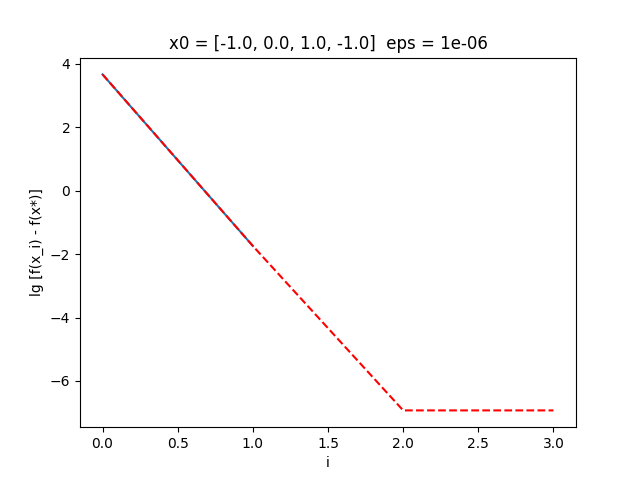
\includegraphics[width=0.9\linewidth]{Figure_6_4}}  \\
	\end{minipage}
\end{sidewaysfigure}

\rotatebox{90}{
	\begin{minipage}{1.55\linewidth}
		\begin{table}[H]
		\caption{}
			\begin{center}
				\begin{tabular}{|c|c|c|c|c|c|c|}
					\hline
					$\varepsilon$ & $x_0$ & $f(x_0)$ & Метод мінімізації & $x^* \text{ - отриманий розв'язок} $  & $f(x^*)$ & Кількість ітерацій \\
					\hline
					\multirow{8}{*}{$10^{-8}$} & \multirow{2}{*}{[2.7, 90, 1500, 10]} & \multirow{2}{*}{28580.05} & 4 кроковий & [   -0.007     4.95  1492.2   388.9] & -69910.58 & 33 \\
					\hhline{~~~----} & & & 3 кроковий & [   -0.0001    -8.1001  1403   696.4] & -69975.01 & 86 \\
					\hhline{~------}
					& \multirow{2}{*}{[2, 140, 1707, 31]} & \multirow{2}{*}{-8899.54} & 4 кроковий & [   -0.003 -32.08  1702.15   590.31] & -69940.02 & 28 \\
					\hhline{~~~----} & & & 3 кроковий & [   -0.00018    -3.7  1679.4   1104.8] & -69985.9 & 88 \\
					\hhline{~------}
					& \multirow{2}{*}{[1, 1, 1, 1]} & \multirow{2}{*}{-65340.91} & 4 кроковий & [ 0.       0.00001  0.005  1.006] & -70000.0 & 8 \\
					\hhline{~~~----} & & & 3 кроковий & [-0.       0.00001  0.001  1.006] & -70000.0 & 7 \\
					\hhline{~------}
					& \multirow{2}{*}{[-1, 0, 1, -1]} & \multirow{2}{*}{-65346.95247} & 4 кроковий & [-0.00001  0.       0.00001 -1.005] & -70000.0 & 4 \\
					\hhline{~~~----} & & & 3 кроковий & [ 0.       0.       0.      -1.00519] & -70000.0 & 4 \\
					\hline	
				\end{tabular}
			\end{center}
		\end{table}
\end{minipage}} 

\begin{sidewaysfigure}
\centering
\caption{}
	\begin{minipage}[h]{0.47\linewidth}
		\center{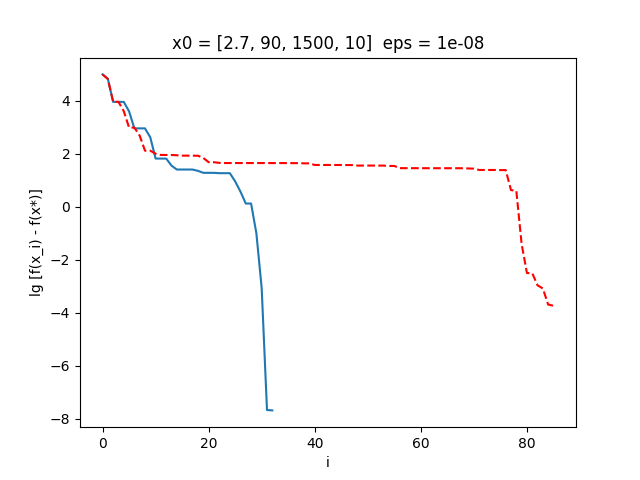
\includegraphics[width=0.9\linewidth]{Figure_6_1_1} \\
	\end{minipage}
	\hfill
	\begin{minipage}[h]{0.47\linewidth}
		\center{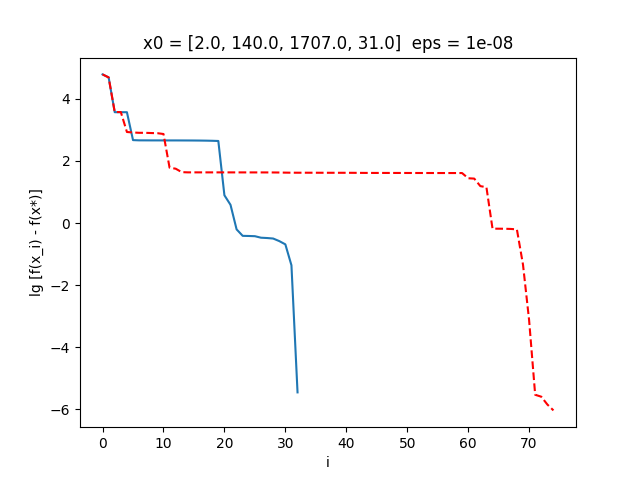
\includegraphics[width=0.9\linewidth]{Figure_6_1_2}} \\
	\end{minipage}
	\vfill
	\begin{minipage}[h]{0.47\linewidth}
		\center{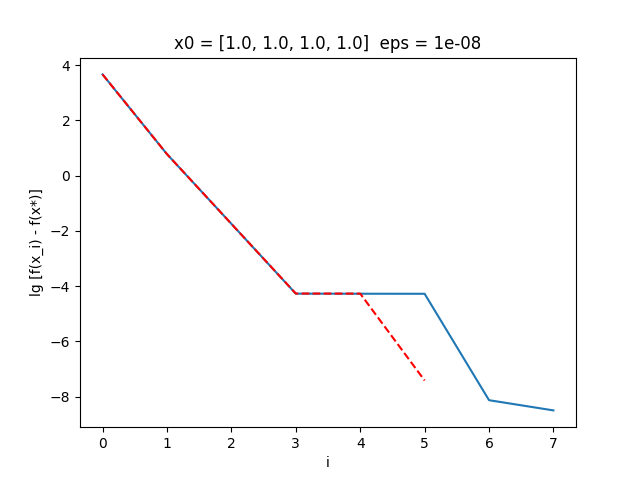
\includegraphics[width=0.9\linewidth]{Figure_6_1_3}}  \\
	\end{minipage}
	\hfill
	\begin{minipage}[h]{0.47\linewidth}
		\center{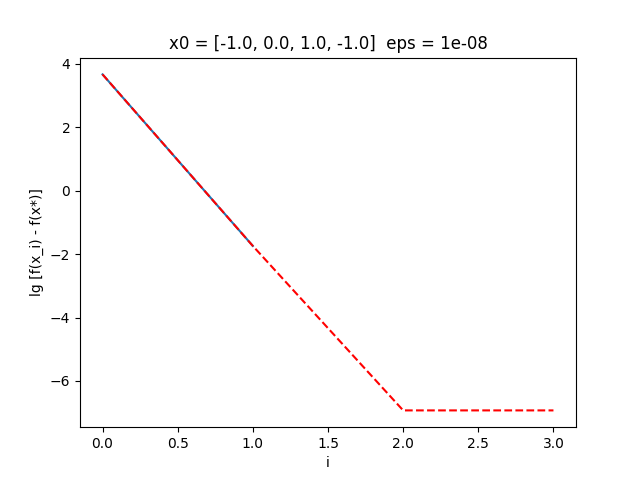
\includegraphics[width=0.9\linewidth]{Figure_6_1_4}}  \\
	\end{minipage}
\end{sidewaysfigure}


\rotatebox{90}{
	\begin{minipage}{1.5\linewidth}
	    \begin{example}
        	$$\phi(x) = \left(- x_{1} \left(- x_{2} + 1\right) + 1.5\right)^{2} + \left(- x_{1} \left(- x_{2}^{2} + 1\right) + 2.25\right)^{2} + \left(- x_{1} \left(- x_{2}^{3} + 1\right) + 2.625\right)^{2}$$
        	Точний розв'язок задачі: x* = [3, 0.5] f* = 0
        \end{example}
		\begin{table}[H]
		\caption{}
			\begin{center}
				\begin{tabular}{|c|c|c|c|c|c|c|}
					\hline
					$\varepsilon$ & $x_0$ & $f(x_0)$ & Метод мінімізації & $x^* \text{ - отриманий розв'язок} $  & $f(x^*)$ & Кількість ітерацій \\
					\hline
					\multirow{8}{*}{$10^{-6}$} & \multirow{2}{*}{[2, 0.2]} & \multirow{2}{*}{0.52978} & 4 кроковий & [ 3.01226  0.50475] & 9e-05 & 27\\
                    \hhline{~~~----} & & & 3 кроковий & [ 2.99704  0.49901] & 0.0 & 13 \\
                    \hhline{~------}
					& \multirow{2}{*}{[1.0, 1.0]} & \multirow{2}{*}{14.20313} & 4 кроковий & [ 2.99354  0.49768] & 2e-05 & 42\\
                    \hhline{~~~----} & & & 3 кроковий & [ 3.00004  0.5    ] & 0.0 & 15 \\ 
                    \hhline{~------}
                    & \multirow{2}{*}{[1.5, 1.5]} & \multirow{2}{*}{60.36328} & 4 кроковий & [ 4.53484  0.72223] & 0.10485 & 14\\
                    \hhline{~~~----} & & & 3 кроковий & [ 2.99818  0.4995 ] & 0.0 & 12 \\ 
                    \hhline{~------}
                    & \multirow{2}{*}{[3.2, -0.1]} & \multirow{2}{*}{5.25744} & 4 кроковий & [ 2.98676  0.49898] & 0.00015 & 3\\
                    \hhline{~~~----} & & & 3 кроковий & [ 2.98676  0.49898] & 0.00015 & 3 \\ 
					\hline	
				\end{tabular}
			\end{center}
		\end{table}
\end{minipage}} 

\begin{sidewaysfigure}
\centering
\caption{}
	\begin{minipage}[h]{0.47\linewidth}
		\center{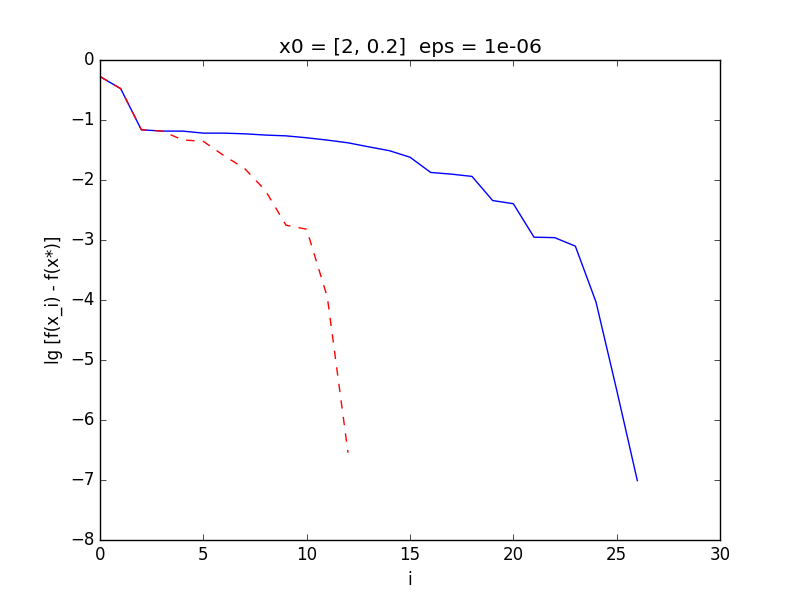
\includegraphics[width=0.9\linewidth]{figure_7_1} \\
	\end{minipage}
	\hfill
	\begin{minipage}[h]{0.47\linewidth}
		\center{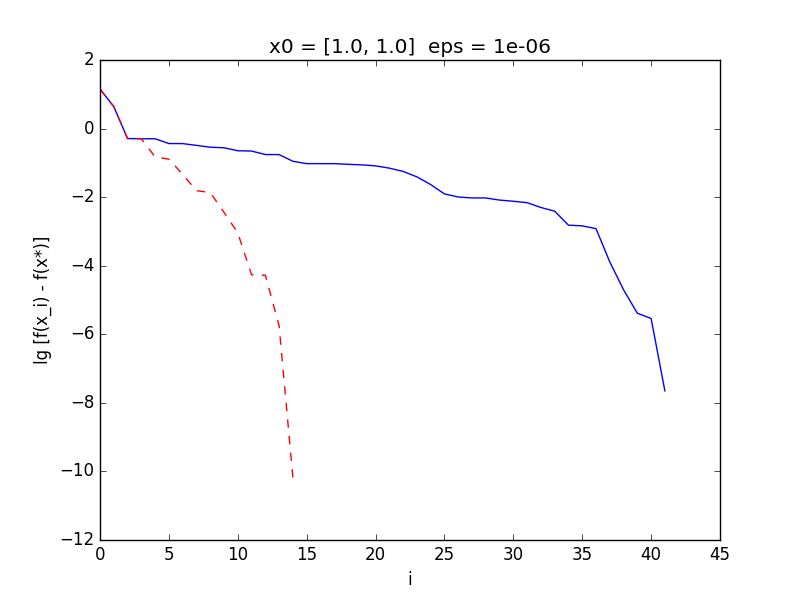
\includegraphics[width=0.9\linewidth]{figure_7_2}} \\
	\end{minipage}
	\vfill
	\begin{minipage}[h]{0.47\linewidth}
		\center{\includegraphics[width=0.9\linewidth]{figure_7_3}}  \\
	\end{minipage}
	\hfill
	\begin{minipage}[h]{0.47\linewidth}
		\center{\includegraphics[width=0.9\linewidth]{figure_7_4}}  \\
	\end{minipage}
\end{sidewaysfigure}

\newpage
\rotatebox{90}{
	\begin{minipage}{1.5\linewidth}
		\begin{table}[H]
		\caption{}
			\begin{center}
				\begin{tabular}{|c|c|c|c|c|c|c|}
					\hline
					$\varepsilon$ & $x_0$ & $f(x_0)$ & Метод мінімізації & $x^* \text{ - отриманий розв'язок} $  & $f(x^*)$ & Кількість ітерацій \\
					\hline
					\multirow{8}{*}{$10^{-8}$} & \multirow{2}{*}{[2, 0.2]} & \multirow{2}{*}{0.52978} & 4 кроковий & [ 2.99785  0.49975] & 0.0 & 32\\
                    \hhline{~~~----} & & & 3 кроковий & [ 2.99979  0.49992] & 0.0 & 17 \\
                    \hhline{~------}
					& \multirow{2}{*}{[1.0, 1.0]} & \multirow{2}{*}{14.20313} & 4 кроковий & [ 2.99996  0.5    ] & 0.0 & 48\\
                    \hhline{~~~----} & & & 3 кроковий & [ 3.00004  0.5    ] & 0.0 & 15 \\ 
                    \hhline{~------}
                    & \multirow{2}{*}{[1.5, 1.5]} & \multirow{2}{*}{60.36328} & 4 кроковий & [ 3.00028  0.50053] & 0.0 & 64\\
                    \hhline{~~~----} & & & 3 кроковий  & [ 3.00014  0.50003] & 0.0 & 18 \\ 
                    \hhline{~------}
                    & \multirow{2}{*}{[3.2, -0.1]} & \multirow{2}{*}{5.25744} & 4 кроковий & [ 2.98676  0.49898] & 0.00015 & 4\\
                    \hhline{~~~----} & & & 3 кроковий & [ 2.99921  0.49981] & 0.0 & 12 \\ 
					\hline	
				\end{tabular}
			\end{center}
		\end{table}
\end{minipage}} 

\begin{sidewaysfigure}
\centering
\caption{}
	\begin{minipage}[h]{0.47\linewidth}
		\center{\includegraphics[width=0.9\linewidth]{figure_7_1_1} \\
	\end{minipage}
	\hfill
	\begin{minipage}[h]{0.47\linewidth}
		\center{\includegraphics[width=0.9\linewidth]{figure_7_1_2}} \\
	\end{minipage}
	\vfill
	\begin{minipage}[h]{0.47\linewidth}
		\center{\includegraphics[width=0.9\linewidth]{figure_7_1_3}}  \\
	\end{minipage}
	\hfill
	\begin{minipage}[h]{0.47\linewidth}
		\center{\includegraphics[width=0.9\linewidth]{figure_7_1_4}}  \\
	\end{minipage}
\end{sidewaysfigure}


\rotatebox{90}{
	\begin{minipage}{1.5\linewidth}
	    \begin{example}
        	$$\phi(x) = \left(- x_{1} + 1\right)^{2} + \left(- x_{1}^{2} + x_{2}\right)^{2}$$
        	Точний розв'язок задачі: x* = [1, 1] f* = 0
        \end{example}
		\begin{table}[H]
		\caption{}
			\begin{center}
				\begin{tabular}{|c|c|c|c|c|c|c|}
					\hline
					$\varepsilon$ & $x_0$ & $f(x_0)$ & Метод мінімізації & $x^* \text{ - отриманий розв'язок} $  & $f(x^*)$ & Кількість ітерацій \\
					\hline
					\multirow{8}{*}{$10^{-6}$} & \multirow{2}{*}{[-1.2, 1]} & \multirow{2}{*}{5.0336} & 4 кроковий & [ 1.00416  1.00311] & 4e-05 & 3\\
                    \hhline{~~~----} & & & 3 кроковий & [ 1.00416  1.00311] & 4e-05 & 3 \\ 
                    \hhline{~------}
					& \multirow{2}{*}{[1.0, -1.2]} & \multirow{2}{*}{4.84} & 4 кроковий & [ 0.98778  0.97715] & 0.00015 & 15\\
                    \hhline{~~~----} & & & 3 кроковий & [ 1.0495   1.11224] & 0.00257 & 8 \\ 
                    \hhline{~------}
                    & \multirow{2}{*}{[-0.5, 1.7]} & \multirow{2}{*}{4.3525} & 4 кроковий & [ 0.94119  0.91092] & 0.00409 & 13\\
                    \hhline{~~~----} & & & 3кроковий  & [ 0.99948  0.99726] & 0.0 & 12 \\ 
                    \hhline{~------}
                    & \multirow{2}{*}{[-1.0, -1.0]} & \multirow{2}{*}{8.0} & 4 кроковий  & [ 0.99152  0.98493] & 8e-05 & 14\\
                    \hhline{~~~----} & & & 3 кроковий & [ 0.98296  0.96712] & 0.00029 & 9 \\
					\hline	
				\end{tabular}
			\end{center}
		\end{table}
\end{minipage}} 

\begin{sidewaysfigure}
\centering
\caption{}
	\begin{minipage}[h]{0.47\linewidth}
		\center{\includegraphics[width=0.9\linewidth]{figure_8_1} \\
	\end{minipage}
	\hfill
	\begin{minipage}[h]{0.47\linewidth}
		\center{\includegraphics[width=0.9\linewidth]{figure_8_2}} \\
	\end{minipage}
	\vfill
	\begin{minipage}[h]{0.47\linewidth}
		\center{\includegraphics[width=0.9\linewidth]{figure_8_3}}  \\
	\end{minipage}
	\hfill
	\begin{minipage}[h]{0.47\linewidth}
		\center{\includegraphics[width=0.9\linewidth]{figure_8_4}}  \\
	\end{minipage}
\end{sidewaysfigure}


\rotatebox{90}{
	\begin{minipage}{1.5\linewidth}
		\begin{table}[H]
		\caption{}
			\begin{center}
				\begin{tabular}{|c|c|c|c|c|c|c|}
					\hline
					$\varepsilon$ & $x_0$ & $f(x_0)$ & Метод мінімізації & $x^* \text{ - отриманий розв'язок} $  & $f(x^*)$ & Кількість ітерацій \\
					\hline
					\multirow{8}{*}{$10^{-8}$} & \multirow{2}{*}{[-1.2, 1]} & \multirow{2}{*}{5.0336} & 4 кроковий & [ 1.00415  1.0031 ] & 4e-05 & 4\\
                    \hhline{~~~----} & & & 3 кроковий & [ 0.99991  1.00003] & 0.0 & 8 \\ 
                    \hhline{~------}
					& \multirow{2}{*}{[1.0, -1.2]} & \multirow{2}{*}{4.84} & 4 кроковий & [ 1.00018  1.00065] & 0.0 & 25\\
                    \hhline{~~~----} & & & 3 кроковий & [ 1.00029  1.00066] & 0.0 & 19 \\ 
                    \hhline{~------}
                    & \multirow{2}{*}{[-0.5, 1.7]} & \multirow{2}{*}{4.3525} & 4 кроковий & [ 0.99986  0.99981] & 0.0 & 25\\
                    \hhline{~~~----} & & & 3 кроковий & [ 0.99999  0.99984] & 0.0 & 16 \\ 
                    \hhline{~------}
                    & \multirow{2}{*}{[-1.0, -1.0]} & \multirow{2}{*}{8.0} & 4 кроковий & [ 1.00036  1.00104] & 0.0 & 21\\
                    \hhline{~~~----} & & & 3 кроковий & [ 0.98296  0.96712] & 0.00029 & 9 \\
					\hline	
				\end{tabular}
			\end{center}
		\end{table}
\end{minipage}} 

\begin{sidewaysfigure}
\centering
\caption{}
	\begin{minipage}[h]{0.47\linewidth}
		\center{\includegraphics[width=0.9\linewidth]{figure_8_1_1} \\
	\end{minipage}
	\hfill
	\begin{minipage}[h]{0.47\linewidth}
		\center{\includegraphics[width=0.9\linewidth]{figure_8_1_2}} \\
	\end{minipage}
	\vfill
	\begin{minipage}[h]{0.47\linewidth}
		\center{\includegraphics[width=0.9\linewidth]{figure_8_1_3}}  \\
	\end{minipage}
	\hfill
	\begin{minipage}[h]{0.47\linewidth}
		\center{\includegraphics[width=0.9\linewidth]{figure_8_1_4}}  \\
	\end{minipage}
\end{sidewaysfigure}

\rotatebox{90}{
	\begin{minipage}{1.5\linewidth}
	    \begin{example}
        	$$\phi(x) = 100 \left(- x_{1} + 1\right)^{2} + \left(- x_{1}^{2} + x_{2}\right)^{2}$$
        	Точний розв'язок задачі: x* = [1, 1] f* = 0
        \end{example}
		\begin{table}[H]
		\caption{}
			\begin{center}
				\begin{tabular}{|c|c|c|c|c|c|c|}
					\hline
					$\varepsilon$ & $x_0$ & $f(x_0)$ & Метод мінімізації & $x^* \text{ - отриманий розв'язок} $  & $f(x^*)$ & Кількість ітерацій \\
					\hline
					\multirow{8}{*}{$10^{-6}$} & \multirow{2}{*}{[-1.2, 1]} & \multirow{2}{*}{484.1936} & 4 кроковий & [ 1.  1.] & 0.0 & 3\\
                    \hhline{~~~----} & & & 3 кроковий & [ 1.  1.] & 0.0 & 3 \\ 
                    \hhline{~------}
					& \multirow{2}{*}{[1.0, -1.2]} & \multirow{2}{*}{4.84} & 4 кроковий & [ 0.99818  1.00144] & 0.00036 & 3\\
                    \hhline{~~~----} & & & 3 кроковий & [ 0.99818  1.00144] & 0.00036 & 3 \\ 
                    \hhline{~------}
                    & \multirow{2}{*}{[-0.5, 1.7]} & \multirow{2}{*}{227.1025} & 4 кроковий  & [ 0.99983  1.00001] & 0.0 & 3\\
                    \hhline{~~~----} & & & 3 кроковий  & [ 0.99983  1.00001] & 0.0 & 3 \\ 
                    \hhline{~------}
                    & \multirow{2}{*}{[-1.0, -1.0]} & \multirow{2}{*}{404.0} & 4 кроковий & [ 0.99872  0.99977] & 0.00017 & 3\\
                    \hhline{~~~----} & & & 3 кроковий & [ 0.99872  0.99977] & 0.00017 & 3 \\
					\hline	
				\end{tabular}
			\end{center}
		\end{table}
\end{minipage}} 

\begin{sidewaysfigure}
\centering
\caption{}
	\begin{minipage}[h]{0.47\linewidth}
		\center{\includegraphics[width=0.9\linewidth]{figure_9_1} \\
	\end{minipage}
	\hfill
	\begin{minipage}[h]{0.47\linewidth}
		\center{\includegraphics[width=0.9\linewidth]{figure_9_2}} \\
	\end{minipage}
	\vfill
	\begin{minipage}[h]{0.47\linewidth}
		\center{\includegraphics[width=0.9\linewidth]{figure_9_3}}  \\
	\end{minipage}
	\hfill
	\begin{minipage}[h]{0.47\linewidth}
		\center{\includegraphics[width=0.9\linewidth]{figure_9_4}}  \\
	\end{minipage}
\end{sidewaysfigure}

\rotatebox{90}{
	\begin{minipage}{1.5\linewidth}
		\begin{table}[H]
		\caption{}
			\begin{center}
				\begin{tabular}{|c|c|c|c|c|c|c|}
					\hline
					$\varepsilon$ & $x_0$ & $f(x_0)$ & Метод мінімізації & $x^* \text{ - отриманий розв'язок} $  & $f(x^*)$ & Кількість ітерацій \\
					\hline
					\multirow{8}{*}{$10^{-8}$} & \multirow{2}{*}{[-1.2, 1]} & \multirow{2}{*}{484.1936} & 4 кроковий & [ 1.  1.] & 0.0 & 3\\
                    \hhline{~~~----} & & & 3 кроковий & [ 1.  1.] & 0.0 & 3 \\ 
                    \hhline{~------}
                    & \multirow{2}{*}{[1.0, -1.2]} & \multirow{2}{*}{4.84} & 4 кроковий & [ 0.99818  1.00145] & 0.00036 & 4\\
                    \hhline{~~~----} & & & 3 кроковий & [ 1.00001  0.99997] & 0.0 & 6 \\ 
                    \hhline{~------}
                    & \multirow{2}{*}{[-0.5, 1.7]} & \multirow{2}{*}{227.1025} & 4 кроковий & [ 0.99983  1.00001] & 0.0 & 3\\
                    \hhline{~~~----} & & & 3 кроковий & [ 0.99983  1.00001] & 0.0 & 3 \\ 
                    \hhline{~------}
                    & \multirow{2}{*}{[-1.0, -1.0]} & \multirow{2}{*}{404.0} & 4 кроковий & [ 0.99872  0.99977] & 0.00017 & 3\\
                    \hhline{~~~----} & & & 3 кроковий & [ 0.99872  0.99977] & 0.00017 & 3 \\				
					\hline	
				\end{tabular}
			\end{center}
		\end{table}
\end{minipage}} 

\begin{sidewaysfigure}
\centering
\caption{}
	\begin{minipage}[h]{0.47\linewidth}
		\center{\includegraphics[width=0.9\linewidth]{figure_9_1_1} \\
	\end{minipage}
	\hfill
	\begin{minipage}[h]{0.47\linewidth}
		\center{\includegraphics[width=0.9\linewidth]{figure_9_1_2}} \\
	\end{minipage}
	\vfill
	\begin{minipage}[h]{0.47\linewidth}
		\center{\includegraphics[width=0.9\linewidth]{figure_9_1_3}}  \\
	\end{minipage}
	\hfill
	\begin{minipage}[h]{0.47\linewidth}
		\center{\includegraphics[width=0.9\linewidth]{figure_9_1_4}}  \\
	\end{minipage}
\end{sidewaysfigure}

\rotatebox{90}{
	\begin{minipage}{1.5\linewidth}
	    \begin{example}
        	$$\phi(x) = \left(- x_{1} + 1\right)^{2} + 100 \left(- x_{1}^{3} + x_{2}\right)^{2}$$
        	Точний розв'язок задачі: x* = [1, 1] f* = 0
        \end{example}
		\begin{table}[H]
		\caption{}
			\begin{center}
				\begin{tabular}{|c|c|c|c|c|c|c|}
					\hline
					$\varepsilon$ & $x_0$ & $f(x_0)$ & Метод мінімізації & $x^* \text{ - отриманий розв'язок} $  & $f(x^*)$ & Кількість ітерацій \\
					\hline
					\multirow{8}{*}{$10^{-6}$} & \multirow{2}{*}{[-1.2, 1]} & \multirow{2}{*}{749.0384} & 4 кроковий & [ 1.00006  1.00002] & 0.0 & 47\\
                    \hhline{~~~----} & & & 3 кроковий & [ 1.01616  1.04847] & 0.00033 & 13 \\ 
                    \hhline{~------}
                    & \multirow{2}{*}{[1.0, -1.2]} & \multirow{2}{*}{484.0} & 4 кроковий & [ 0.72054  0.37033] & 0.07951 & 14\\
                    \hhline{~~~----} & & & 3 кроковий & [ 0.99952  0.99839] & 0.0 & 28 \\ 
                    \hhline{~------}
					& \multirow{2}{*}{[-0.5, 1.7]} & \multirow{2}{*}{335.3125} & 4 кроковий & [ 0.99958  0.99876] & 0.0 & 58\\
                    \hhline{~~~----} & & & 3 кроковий & [ 0.99993  0.99958] & 0.0 & 21 \\ 
                    \hhline{~------}
                    & \multirow{2}{*}{[-1.0, -1.0]} & \multirow{2}{*}{4.0} & 4 кроковий & [ 1.51124  3.4527 ] & 0.26153 & 11\\
                    \hhline{~~~----} & & & 3 кроковий & [ 1.00105  1.00325] & 0.0 & 32 \\ 
					\hline	
				\end{tabular}
			\end{center}
		\end{table}
\end{minipage}} 

\begin{sidewaysfigure}
\centering
\caption{}
	\begin{minipage}[h]{0.47\linewidth}
		\center{\includegraphics[width=0.9\linewidth]{figure_10_1} \\
	\end{minipage}
	\hfill
	\begin{minipage}[h]{0.47\linewidth}
		\center{\includegraphics[width=0.9\linewidth]{figure_10_2}} \\
	\end{minipage}
	\vfill
	\begin{minipage}[h]{0.47\linewidth}
		\center{\includegraphics[width=0.9\linewidth]{figure_10_3}}  \\
	\end{minipage}
	\hfill
	\begin{minipage}[h]{0.47\linewidth}
		\center{\includegraphics[width=0.9\linewidth]{figure_10_4}}  \\
	\end{minipage}
\end{sidewaysfigure}

\rotatebox{90}{
	\begin{minipage}{1.5\linewidth}
		\begin{table}[H]
		\caption{}
			\begin{center}
				\begin{tabular}{|c|c|c|c|c|c|c|}
					\hline
					$\varepsilon$ & $x_0$ & $f(x_0)$ & Метод мінімізації & $x^* \text{ - отриманий розв'язок} $  & $f(x^*)$ & Кількість ітерацій \\
					\hline
					\multirow{8}{*}{$10^{-8}$} & \multirow{2}{*}{[-1.2, 1]} & \multirow{2}{*}{749.0384} & 4 кроковий & [ 0.99997  0.99987] & 0.0 & 51\\
                    \hhline{~~~----} & & & 3 кроковий & [ 1.00012  1.00037] & 0.0 & 24 \\ 
                    \hhline{~------}
					& \multirow{2}{*}{[1.0, -1.2]} & \multirow{2}{*}{484.0} & 4 кроковий  & [ 1.00001  1.00002] & 0.0 & 52\\
                    \hhline{~~~----} & & & 3 кроковий & [ 1.00017  1.00052] & 0.0 & 32 \\ 
                    \hhline{~------}
                    & \multirow{2}{*}{[-0.5, 1.7]} & \multirow{2}{*}{335.3125} & 4 кроковий & [ 0.99959  0.99878] & 0.0 & 59\\
                    \hhline{~~~----} & & & 3 кроковий & [ 1.00003  1.00009] & 0.0 & 24 \\ 
                    \hhline{~------}
                    & \multirow{2}{*}{[-1.0, -1.0]} & \multirow{2}{*}{4.0} & 4 кроковий & [ 1.00026  1.0007 ] & 0.0 & 75\\
                    \hhline{~~~----} & & & 3 кроковий & [ 1.00002  1.00005] & 0.0 & 36 \\ 
					\hline	
				\end{tabular}
			\end{center}
		\end{table}
\end{minipage}} 

\begin{sidewaysfigure}
\centering
\caption{}
	\begin{minipage}[h]{0.47\linewidth}
		\center{\includegraphics[width=0.9\linewidth]{figure_10_1_1} \\
	\end{minipage}
	\hfill
	\begin{minipage}[h]{0.47\linewidth}
		\center{\includegraphics[width=0.9\linewidth]{figure_10_1_2}} \\
	\end{minipage}
	\vfill
	\begin{minipage}[h]{0.47\linewidth}
		\center{\includegraphics[width=0.9\linewidth]{figure_10_1_3}}  \\
	\end{minipage}
	\hfill
	\begin{minipage}[h]{0.47\linewidth}
		\center{\includegraphics[width=0.9\linewidth]{figure_10_1_4}}  \\
	\end{minipage}
\end{sidewaysfigure}

\rotatebox{90}{
	\begin{minipage}{1.56\linewidth}
	    \begin{example}
        	$$\phi(x) = - 90 x_{3}^{2} + 90 x_{4} + \left(- x_{1} + 1\right)^{2} + 100 \left(- x_{1}^{2} + x_{2}\right)^{2} + 10.1 \left(x_{2} - 1\right)^{2} + \left(19.8 x_{2} - 19.8\right) \left(x_{4} - 1\right) + \left(- x_{3} + 1\right)^{3} + 10.1 \left(x_{4} - 1\right)^{2}$$
        	Точний розв'язок задачі: x* = [1, 1, 1, 1] f* = 0
        \end{example}
		\begin{table}[H]
		\caption{}
			\begin{center}
				\begin{tabular}{|c|c|c|c|c|c|c|}
					\hline
					$\varepsilon$ & $x_0$ & $f(x_0)$ & Метод мінімізації & $x^* \text{ - отриманий розв'язок} $  & $f(x^*)$ & Кількість ітерацій \\
					\hline
					\multirow{8}{*}{$10^{-6}$} & \multirow{2}{*}{[1, 0, 1, 0]} & \multirow{2}{*}{50.0} & 4 кроковий & [  -893.1  23070.9  39658.05  -8493.8] & -2.5e+12 & 40\\
                    \hhline{~~~----} & & & 3 кроковий & [  -2498.5   92057.4  158263.3  -33891.8] & -1.8e+14 & 37 \\ 
                    \hhline{~------}
                    & \multirow{2}{*}{[0, 0, 0, 0]} & \multirow{2}{*}{42.0} & 4 кроковий & [   3237.4   47239.3  226062.6 -274971.1] & -6.7e+14 & 63\\
                    \hhline{~~~----} & & & 3 кроковий & [   2796  45589  183703   -233672.2] & -1.5e+14 & 48 \\ 
                    \hhline{~------}
                    & \multirow{2}{*}{[-0.2, 0.5, 1, 0]} & \multirow{2}{*}{-44.875} & 4 кроковий & [ -141.8 -1118.2   3577.9 -1152.2] & -1789598322 & 24\\
                    \hhline{~~~----} & & & 3 кроковий & [  -4215  -99475  318541 -102514] & -3.8e+14 & 39 \\ 
                    \hhline{~------}
        			& \multirow{2}{*}{[-1, -1, -1, -1]} & \multirow{2}{*}{392} & 4 кроковий & [   894.8   3201.2  40997.3  -27920.8] & -5.4e+12 & 61\\
                    \hhline{~~~----} & & & 3 кроковий & [  2.7e+06  0   1.9e+09  -1.7e+08] & -1.8e+27 & 49 \\		
					\hline	
				\end{tabular}
			\end{center}
		\end{table}
\end{minipage}} 

\begin{sidewaysfigure}
\centering
\caption{}
	\begin{minipage}[h]{0.47\linewidth}
		\center{\includegraphics[width=0.9\linewidth]{figure_11_1} \\
	\end{minipage}
	\hfill
	\begin{minipage}[h]{0.47\linewidth}
		\center{\includegraphics[width=0.9\linewidth]{figure_11_2}} \\
	\end{minipage}
	\vfill
	\begin{minipage}[h]{0.47\linewidth}
		\center{\includegraphics[width=0.9\linewidth]{figure_11_3}}  \\
	\end{minipage}
	\hfill
	\begin{minipage}[h]{0.47\linewidth}
		\center{\includegraphics[width=0.9\linewidth]{figure_11_4}}  \\
	\end{minipage}
\end{sidewaysfigure}

\rotatebox{90}{
	\begin{minipage}{1.55\linewidth}
		\begin{table}[H]
		\caption{}
			\begin{center}
				\begin{tabular}{|c|c|c|c|c|c|c|}
					\hline
					$\varepsilon$ & $x_0$ & $f(x_0)$ & Метод мінімізації & $x^* \text{ - отриманий розв'язок} $  & $f(x^*)$ & Кількість ітерацій \\
					\hline
					\multirow{8}{*}{$10^{-8}$} & \multirow{2}{*}{[1, 0, 1, 0]} & \multirow{2}{*}{50.0} & 4 кроковий & [  -893.12  23070.94 39658.05  -8493.82] & -2.50e+12 & 40\\
                    \hhline{~~~----} & & & 3 кроковий & [  -2498.5   92057.4  158263.3  -33891.84] & -1.84e+14 & 37 \\ 
                    \hhline{~------}
                    & \multirow{2}{*}{[0, 0, 0, 0]} & \multirow{2}{*}{42.0} & 4 кроковий & [   3237.45   47239.37  226062.61 -274971] & -6.70e+14 & 63\\
                    \hhline{~~~----} & & & 3 кроковий & [   2796.1   45589  183703   -233672] & -1.598e+14 & 48 \\ 
                    \hhline{~------}
                    & \multirow{2}{*}{[-0.2, 0.5, 1, 0]} & \multirow{2}{*}{-44.8} & 4 кроковий & [ -141.8 -1118.2   3577.94 -1152.22] & -178959832 & 24\\
                    \hhline{~~~----} & & & 3 кроковий & [  -4215.83  -99475.2  318541.8 -102513.87] & -3.86e+14 & 39 \\ 
                    \hhline{~------}
        			& \multirow{2}{*}{[-1, -1, -1, -1]} & \multirow{2}{*}{392.0} & 4 кроковий & [   894.8   3201.2 40997.3 -27920.83] & -5.43e+12 & 61\\
                    \hhline{~~~----} & & & 3 кроковий & [  2.7e+07  -1.5e+08   1.4e+09  -1.1e+08] & -1.8e+27 & 49 \\		
					\hline	
				\end{tabular}
			\end{center}
		\end{table}
\end{minipage}} 

\begin{sidewaysfigure}
\centering
\caption{}
	\begin{minipage}[h]{0.47\linewidth}
		\center{\includegraphics[width=0.9\linewidth]{figure_11_1_1} \\
	\end{minipage}
	\hfill
	\begin{minipage}[h]{0.47\linewidth}
		\center{\includegraphics[width=0.9\linewidth]{figure_11_1_2}} \\
	\end{minipage}
	\vfill
	\begin{minipage}[h]{0.47\linewidth}
		\center{\includegraphics[width=0.9\linewidth]{figure_11_1_3}}  \\
	\end{minipage}
	\hfill
	\begin{minipage}[h]{0.47\linewidth}
		\center{\includegraphics[width=0.9\linewidth]{figure_11_1_4}}  \\
	\end{minipage}
\end{sidewaysfigure}

\rotatebox{90}{
	\begin{minipage}{1.5\linewidth}
	    \begin{example}
        	$$\phi(x) = \left(x_{1} + 40 x_{2}\right)^{2} + 10 \left(x_{1} - x_{4}\right)^{4} + \left(x_{2} - 2 x_{3}\right)^{4} + 5 \left(x_{3} - x_{4}\right)^{2}$$
        	Точний розв'язок задачі: x* = [0, 0, 0, 0] f* = 0
        \end{example}
		\begin{table}[H]
		\caption{}
			\begin{center}
				\begin{tabular}{|c|c|c|c|c|c|c|}
					\hline
					$\varepsilon$ & $x_0$ & $f(x_0)$ & Метод мінімізації & $x^* \text{ - отриманий розв'язок} $  & $f(x^*)$ & Кількість ітерацій \\
					\hline
					\multirow{8}{*}{$10^{-6}$} & \multirow{2}{*}{[-3, -1, 0, 1]} & \multirow{2}{*}{4415} & 4 кроковий & [-0.00905  0.00023  0.022  0.026] & 1e-05 & 61\\
                    \hhline{~~~----} & & & 3 кроковий & [-0.0226   0.00057 -0.00345 -0.0034] & 0.0 & 44 \\ 
                    \hhline{~------}
                    & \multirow{2}{*}{[1, 1, 1, 1]} & \multirow{2}{*}{1682.0} & 4 кроковий & [ 0.02 -0.00075 -0.03 -0.03] & 0.00024 & 37\\
                    \hhline{~~~----} & & & 3 кроковий & [ 0.11  -0.00268  0.04  0.04] & 0.00023 & 35 \\
                    \hhline{~------}
					& \multirow{2}{*}{[-1, 0, 1, 0]} & \multirow{2}{*}{32.0} & 4 кроковий & [-0.09  0.002 -0.04 -0.04] & 0.0002 & 68\\
                    \hhline{~~~----} & & & 3 кроковий  & [ 0.00103 -0.00003 -0.02 -0.023] & 1e-05 & 26 \\ 
                    \hhline{~------}
                    & \multirow{2}{*}{[0.5, -0.3, 1, -1]} & \multirow{2}{*}{230.8591} & 4 кроковий & [-0.081  0.002   -0.04 -0.04] & 8e-05 & 30\\
                    \hhline{~~~----} & & & 3 кроковий & [-0.07  0.002 -0.04 -0.04] & 7e-05 & 28 \\
					\hline	
				\end{tabular}
			\end{center}
		\end{table}
\end{minipage}} 

\begin{sidewaysfigure}
\centering
\caption{}
	\begin{minipage}[h]{0.47\linewidth}
		\center{\includegraphics[width=0.9\linewidth]{figure_12_1} \\
	\end{minipage}
	\hfill
	\begin{minipage}[h]{0.47\linewidth}
		\center{\includegraphics[width=0.9\linewidth]{figure_12_2}} \\
	\end{minipage}
	\vfill
	\begin{minipage}[h]{0.47\linewidth}
		\center{\includegraphics[width=0.9\linewidth]{figure_12_3}}  \\
	\end{minipage}
	\hfill
	\begin{minipage}[h]{0.47\linewidth}
		\center{\includegraphics[width=0.9\linewidth]{figure_12_4}}  \\
	\end{minipage}
\end{sidewaysfigure}

\rotatebox{90}{
	\begin{minipage}{1.5\linewidth}
		\begin{table}[H]
		\caption{}
			\begin{center}
				\begin{tabular}{|c|c|c|c|c|c|c|}
					\hline
					$\varepsilon$ & $x_0$ & $f(x_0)$ & Метод мінімізації & $x^* \text{ - отриманий розв'язок} $  & $f(x^*)$ & Кількість ітерацій \\
					\hline
					\multirow{8}{*}{$10^{-8}$} & \multirow{2}{*}{[-3, -1, 0, 1]} & \multirow{2}{*}{4415.0} & 4 кроковий & [-0.00079  0.00002  0.02  0.02] & 1e-05 & 79\\
                    \hhline{~~~----} & & & 3 кроковий & [-0.022   0.00057 -0.003 -0.003] & 0.0 & 45 \\ 
                    \hhline{~------}
                    & \multirow{2}{*}{[1, 1, 1, 1]} & \multirow{2}{*}{1682.0} & 4 кроковий  & [ 0.0333  -0.00083  0.01378  0.0138 ] & 0.0 & 119\\
                    \hhline{~~~----} & & & 3 кроковий & [-0.00311  0.00008  0.00838  0.0084] & 0.0 & 88 \\ 
                    \hhline{~------}
					& \multirow{2}{*}{[-1, 0, 1, 0]} & \multirow{2}{*}{32.0} & 4 кроковий & [-0.09  0.002  -0.04 -0.05] & 0.0002 & 73\\
                    \hhline{~~~----} & & & 3 кроковий & [-0.00099  0.00002 -0.02171 -0.02171] & 1e-05 & 31 \\ 
                    \hhline{~------}
                    & \multirow{2}{*}{[0.5, -0.3, 1, -1]} & \multirow{2}{*}{230.85} & 4 кроковий & [-0.002  0.00007 -0.02 -0.02] & 1e-05 & 98\\
                    \hhline{~~~----} & & & 3 кроковий & [ 0.001 -0.00004  0.01  0.01] & 0.0 & 134 \\ 
					\hline	
				\end{tabular}
			\end{center}
		\end{table}
\end{minipage}} 

\begin{sidewaysfigure}
\centering
\caption{}
	\begin{minipage}[h]{0.47\linewidth}
		\center{\includegraphics[width=0.9\linewidth]{figure_12_1_1} \\
	\end{minipage}
	\hfill
	\begin{minipage}[h]{0.47\linewidth}
		\center{\includegraphics[width=0.9\linewidth]{figure_12_1_2}} \\
	\end{minipage}
	\vfill
	\begin{minipage}[h]{0.47\linewidth}
		\center{\includegraphics[width=0.9\linewidth]{figure_12_1_3}}  \\
	\end{minipage}
	\hfill
	\begin{minipage}[h]{0.47\linewidth}
		\center{\includegraphics[width=0.9\linewidth]{figure_12_1_4}}  \\
	\end{minipage}
\end{sidewaysfigure}

\rotatebox{90}{
	\begin{minipage}{1.5\linewidth}
	    \begin{example}
        	$$\phi(x) = -exp^{- x_{1}^{2} - 20.25 \left(x_{1} - x_{2}\right)^{2} + 1} x_{1}^{2}$$
        	Точний розв'язок задачі: x* = [1, 1] f* = -1
        \end{example}
		\begin{table}[H]
		\caption{}
			\begin{center}
				\begin{tabular}{|c|c|c|c|c|c|c|}
					\hline
					$\varepsilon$ & $x_0$ & $f(x_0)$ & Метод мінімізації & $x^* \text{ - отриманий розв'язок} $  & $f(x^*)$ & Кількість ітерацій \\
					\hline
            		\multirow{8}{*}{$10^{-6}$} & \multirow{2}{*}{[0.1, 0.1]} & \multirow{2}{*}{-0.02691} & 4 кроковий & [ 0.99989  0.99979] & -1.0 & 19\\
                    \hhline{~~~----} & & & 3 кроковий & [ 0.99901  0.99964] & -0.99999 & 8 \\ 
                    \hhline{~------}
                    & \multirow{2}{*}{[2.0, 2.0]} & \multirow{2}{*}{-0.19915} & 4 кроковий & [ 0.98801  0.99848] & -0.99749 & 4\\
                    \hhline{~~~----} & & & 3 кроковий & [ 1.00018  1.00011] & -1.0 & 5 \\ 
                    \hhline{~------}
                    & \multirow{2}{*}{[0.5, 0.7]} & \multirow{2}{*}{-0.23544} & 4 кроковий & [ 1.00035  1.00048] & -1.0 & 8\\
                    \hhline{~~~----} & & & 3 кроковий & [ 1.  1.] & -1.0 & 7 \\ 
                    \hhline{~------}
                    & \multirow{2}{*}{[1.3, 2.6]} & \multirow{2}{*}{-0.0} & 4 кроковий & [ 0.99831  1.00391] & -0.99936 & 3\\
                    \hhline{~~~----} & & & 3 кроковий  & [ 0.99831  1.00391] & -0.99936 & 3 \\ 
					\hline	
				\end{tabular}
			\end{center}
		\end{table}
\end{minipage}} 

\begin{sidewaysfigure}
\centering
\caption{}
	\begin{minipage}[h]{0.47\linewidth}
		\center{\includegraphics[width=0.9\linewidth]{figure_13_1} \\
	\end{minipage}
	\hfill
	\begin{minipage}[h]{0.47\linewidth}
		\center{\includegraphics[width=0.9\linewidth]{figure_13_2}} \\
	\end{minipage}
	\vfill
	\begin{minipage}[h]{0.47\linewidth}
		\center{\includegraphics[width=0.9\linewidth]{figure_13_3}}  \\
	\end{minipage}
	\hfill
	\begin{minipage}[h]{0.47\linewidth}
		\center{\includegraphics[width=0.9\linewidth]{figure_13_4}}  \\
	\end{minipage}
\end{sidewaysfigure}

\rotatebox{90}{
	\begin{minipage}{1.5\linewidth}
		\begin{table}[H]
		\caption{}
			\begin{center}
				\begin{tabular}{|c|c|c|c|c|c|c|}
					\hline
					$\varepsilon$ & $x_0$ & $f(x_0)$ & Метод мінімізації & $x^* \text{ - отриманий розв'язок} $  & $f(x^*)$ & Кількість ітерацій \\
					\hline
					\multirow{8}{*}{$10^{-8}$} & \multirow{2}{*}{[0.1, 0.1]} & \multirow{2}{*}{-0.02691} & 4 кроковий & [ 0.99987  0.99978] & -1.0 & 20\\
                    \hhline{~~~----} & & & 3 кроковий  & [ 1.00008  1.00008] & -1.0 & 11 \\ 
                    \hhline{~------}
					& \multirow{2}{*}{[2.0, 2.0]} & \multirow{2}{*}{-0.19915} & 4 кроковий & [ 0.99984  0.99987] & -1.0 & 13\\
                    \hhline{~~~----} & & & 3 кроковий & [ 1.00022  1.00016] & -1.0 & 6 \\ 
                    \hhline{~------}
                    & \multirow{2}{*}{[0.5, 0.7]} & \multirow{2}{*}{-0.23544} & 4 кроковий & [ 0.99061  0.99941] & -0.99826 & 4\\
                    \hhline{~~~----} & & & 3 кроковий & [ 1.00005  1.00004] & -1.0 & 10 \\ 
                    \hhline{~------}
                    & \multirow{2}{*}{[1.3, 2.6]} & \multirow{2}{*}{-0.0} & 4 кроковий & [ 0.99831  1.00391] & -0.99936 & 3\\
                    \hhline{~~~----} & & & 3 кроковий & [ 0.99831  1.00391] & -0.99936 & 3 \\ 
					\hline	
				\end{tabular}
			\end{center}
		\end{table}
\end{minipage}} 

\begin{sidewaysfigure}
\centering
\caption{}
	\begin{minipage}[h]{0.47\linewidth}
		\center{\includegraphics[width=0.9\linewidth]{figure_13_1_1} \\
	\end{minipage}
	\hfill
	\begin{minipage}[h]{0.47\linewidth}
		\center{\includegraphics[width=0.9\linewidth]{figure_13_1_2}} \\
	\end{minipage}
	\vfill
	\begin{minipage}[h]{0.47\linewidth}
		\center{\includegraphics[width=0.9\linewidth]{figure_13_1_3}}  \\
	\end{minipage}
	\hfill
	\begin{minipage}[h]{0.47\linewidth}
		\center{\includegraphics[width=0.9\linewidth]{figure_13_1_4}}  \\
	\end{minipage}
\end{sidewaysfigure}




